% The first command in your LaTeX source must be the \documentclass command.
\documentclass[acmlarge,screen,dvipsnames]{acmart}
%\usepackage{color}
\usepackage{amsmath}
\usepackage{pseudocode}
\usepackage[ruled]{algorithm2e}
\usepackage{algorithmicx}
\usepackage{subcaption}
\usepackage{natbib}
%\usepackage{afterpage}  % for float-page placement trick
\usepackage{placeins}

\input widebar

\usepackage[normalem]{ulem}  % for strike-through (\sout)
\input twmacros
%
% defining the \BibTeX command - from Oren Patashnik's original BibTeX documentation.
\def\BibTeX{{\rm B\kern-.05em{\sc i\kern-.025em b}\kern-.08emT\kern-.1667em\lower.7ex\hbox{E}\kern-.125emX}}
 

\setcopyright{acmcopyright}
\acmJournal{JOCCH}
\acmYear{2020} \acmVolume{13} \acmNumber{1} \acmArticle{1} \acmMonth{1} \acmPrice{15.00}\acmDOI{10.1145/3351343}



% \usepackage{balance}
%
% Rights management information. 
% This information is sent to you when you complete the rights form.
% These commands have SAMPLE values in them; it is your responsibility as an author to replace
% the commands and values with those provided to you when you complete the rights form.
%
% These commands are for a PROCEEDINGS abstract or paper.
%\copyrightyear{2018}
%\acmYear{2018}
%\setcopyright{acmlicensed}
%\acmConference[Woodstock '18]{Woodstock '18: ACM Symposium on Neural Gaze Detection}{June 03--05, 2018}{Woodstock, NY}
%\acmBooktitle{Woodstock '18: ACM Symposium on Neural Gaze Detection, June 03--05, 2018, Woodstock, NY}
%\acmPrice{15.00}
%\acmDOI{10.1145/1122445.1122456}
%\acmISBN{978-1-4503-9999-9/18/06}

%
% These commands are for a JOURNAL article.

% \setcopyright{acmcopyright}
% \acmJournal{JOCCH}
% \acmYear{2020} \acmVolume{13} \acmNumber{1} \acmArticle{1} \acmMonth{1} \acmPrice{15.00}\acmDOI{10.1145/3351343}

%
% Submission ID. 
% Use this when submitting an article to a sponsored event. You'll receive a unique submission ID from the organizers
% of the event, and this ID should be used as the parameter to this command.
%\acmSubmissionID{123-A56-BU3}

%
% The majority of ACM publications use numbered citations and references. If you are preparing content for an event
% sponsored by ACM SIGGRAPH, you must use the "author year" style of citations and references. Uncommenting
% the next command will enable that style.
%\citestyle{acmauthoryear}

%
% end of the preamble, start of the body of the document source.
\begin{document}

%
% The "title" command has an optional parameter, allowing the author to define a "short title" to be used in page headers.

\title[Creative Interactive Experience of Communities' Cultural Heritage via Augmented Reality (AR) Maps]%
      {Creative Interactive Experience of Communities' Cultural Heritage via Augmented Reality (AR) Maps}
%
% The "author" command and its associated commands are used to define the authors and their affiliations.
% Of note is the shared affiliation of the first two authors, and the "authornote" and "authornotemark" commands
% used to denote shared contribution to the research.
% \author{Karina Rodriguez Echavarria}
% \email{K.Rodriguez@brighton.ac.uk}
% \orcid{0000-0002-8679-1602}
% \affiliation{%
%   \institution{Centre for Secure, Intelligent and Usable Systems, University of Brighton}
%   \city{Brighton}
%   \country{United Kingdom}
% }

% \author{Myrsini Samaroudi}
% \affiliation{%
%   \institution{Centre for Secure, Intelligent and Usable Systems, University of Brighton}
%   \city{Brighton}
%   \country{United Kingdom}
%   }

% \author{Tim Weyrich}
% \affiliation{%
%   \institution{Department of Computer Science, University College London}
%   \city{London}
%   \country{United Kingdom}
% }

%
% By default, the full list of authors will be used in the page headers. Often, this list is too long, and will overlap
% other information printed in the page headers. This command allows the author to define a more concise list
% of authors' names for this purpose.
\renewcommand{\shortauthors}{K. Rodriguez, et al.}

%
% A "teaser" image appears between the author and affiliation information and the body 
% of the document, and typically spans the page. 
\begin{teaserfigure}
\centering
 %  \subcaptionbox{Physical creative artwork created by children in the community\label{step1}}
 % {
 % 
 \includegraphics[width=.45\linewidth]{images/mapalone}
 % }
 % \subcaptionbox{Generated Augumented Reality Map with embedded digital elements of the artwork\label{step2}}{
 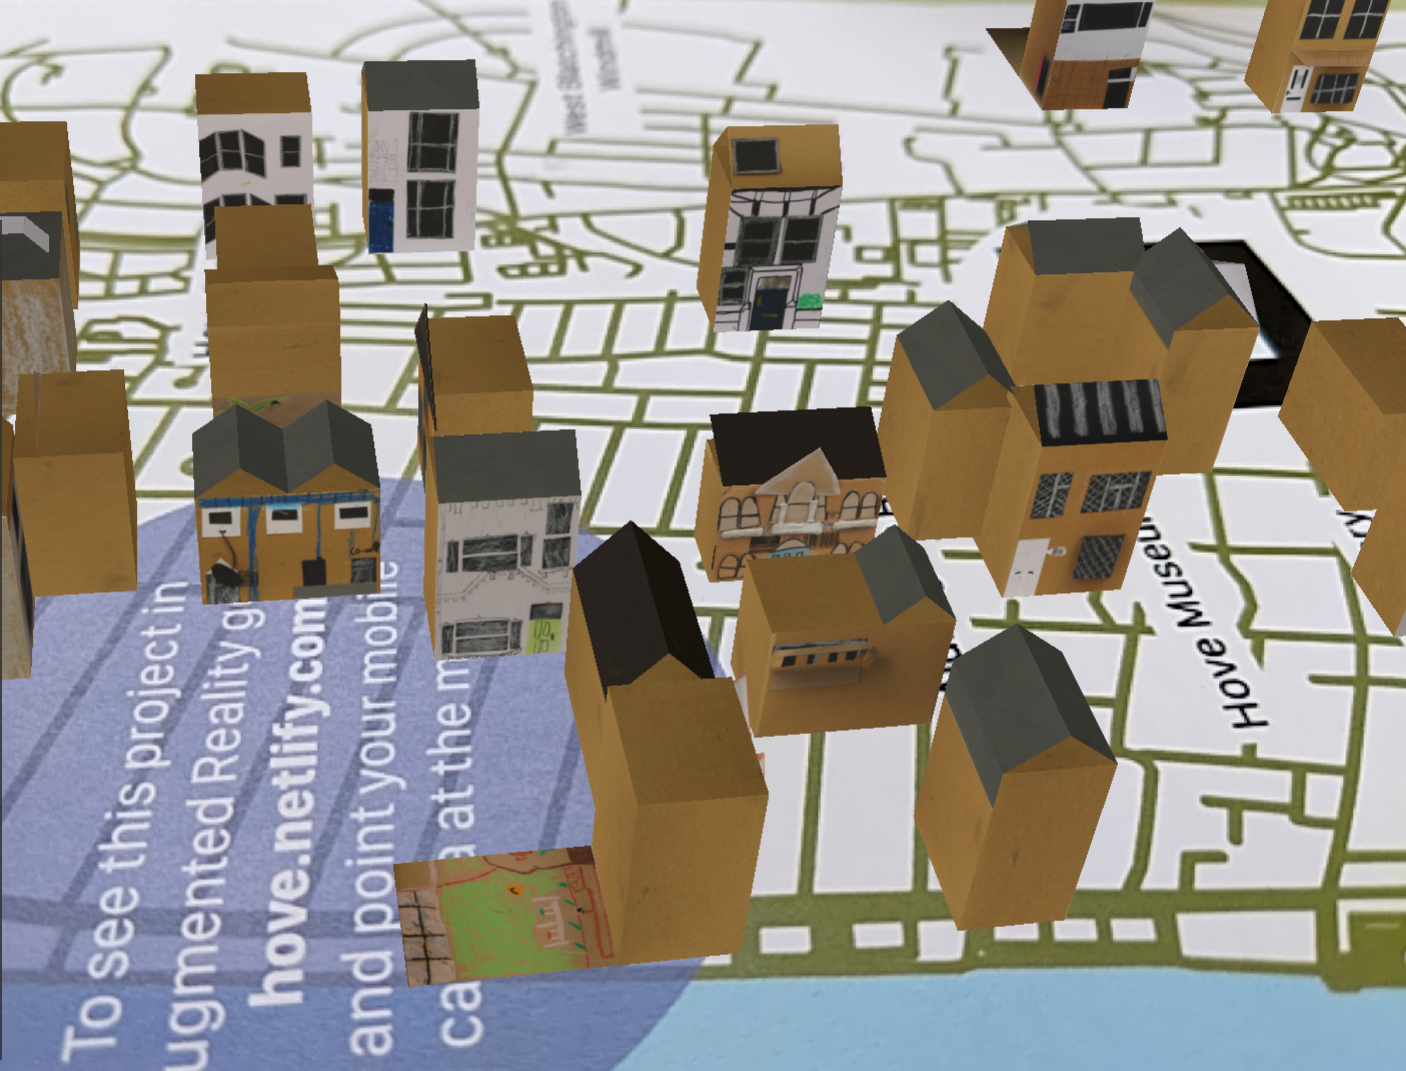
\includegraphics[width=.40\linewidth]{images/screenshoot}
 % }
 % \\[0.5\baselineskip]
  \caption{Artwork and Augmented Reality (AR) Map
with embedded creative narratives of the communities' cultural environment 
for dissemination to a wider audience\vspace*{0.5\baselineskip}}
  \label{fig:teaser}
\end{teaserfigure}


%-------------------------------------------------------------------------
\begin{abstract} This research investigates how communities can
meaningfully connect with Cultural Heritage through creative and digital
experiences. It also explores how entry barriers can be lowered for
a wider set of audiences to increase their participation in such experiences.
For this, the research investigates the use of creative and narrative-based
approaches, given the potential for stories to illuminate different viewpoints
and interpretations of Cultural Heritage within the community. The contribution of the
paper is two fold
contribution is a novel approach for re-telling communities' narratives
linked to people, objects, sites and events in the urban landscape as told by
the community. The research proposed the novel concept of \emph{Augmented
Reality (AR) Maps}, which are physical maps with augmented digital narratives
and delivered through \emph{Immersive Web} technology. This concept is
proposed as a means to document and disseminate the narratives in a way which
can enhance the public understanding and appreciation of objects and sites in
their communities. The approach has been tested with 32 children in local
primary school in the city of Brighton and Hove (UK) in order to understand its suitability
for community engagement. The significance of the research is that it
demonstrates the potential of both creative and digital approaches for
enabling meaningful engagement with the Cultural Heritage, while improving the
well-being of the participants as well as their sense of community and place.
\end{abstract}
%------------------------------------------------------------------------- % 
% ACM CCS 1998 %  (see http://www.acm.org/about/class/1998) %
% \begin{classification} % according to http:http://www.acm.org/about/class/1998
% \CCScat{Computer Graphics}{I.3.3}{Picture/Image Generation}{Line and curve
% generation} % \end{classification}
%------------------------------------------------------------------------- % 
% ACM CCS 2012 %   (see http://www.acm.org/about/class/class/2012) %The tool at
% \url{http://dl.acm.org/ccs.cfm} can be used to generate % CCS codes. %Example:
\begin{CCSXML} <ccs2012> <concept>
<concept_id>10003120.10003121.10003124.10010392</concept_id>
<concept_desc>Human-centered computing~Mixed / augmented
reality</concept_desc> <concept_significance>500</concept_significance>
</concept> <concept>
<concept_id>10002951.10003227.10003236.10003237</concept_id>
<concept_desc>Information systems~Geographic information
systems</concept_desc> <concept_significance>300</concept_significance>
</concept> <concept> <concept_id>10002951.10003260.10003282</concept_id>
<concept_desc>Information systems~Web applications</concept_desc>
<concept_significance>300</concept_significance> </concept> <concept>
<concept_id>10010405.10010469.10010474</concept_id> <concept_desc>Applied
computing~Media arts</concept_desc>
<concept_significance>300</concept_significance> </concept> </ccs2012>
\end{CCSXML}

\ccsdesc[500]{Human-centered computing~Mixed / augmented reality}
\ccsdesc[300]{Information systems~Geographic information systems}
\ccsdesc[300]{Information systems~Web applications} \ccsdesc[300]{Applied
computing~Media arts} 

\maketitle
%-------------------------------------------------------------------------
\section{Introduction} In recent years, the development of graphics
technologies has focused on easing the task of recording, classifying and
preserving cultural assets (e.g. museum objects, heritage buildings). However,
there is a current shift from researching how artefacts might
benefit from these technologies to understanding how communities can
participate in the process of identifying which artefacts to preserve. 


\begin{figure}[b]
  \centering
  \subcaptionbox{Puzzle-pot from the Bristol Museum \& Art Gallery (UK), photo courtesy of Andrew Maxted}
  {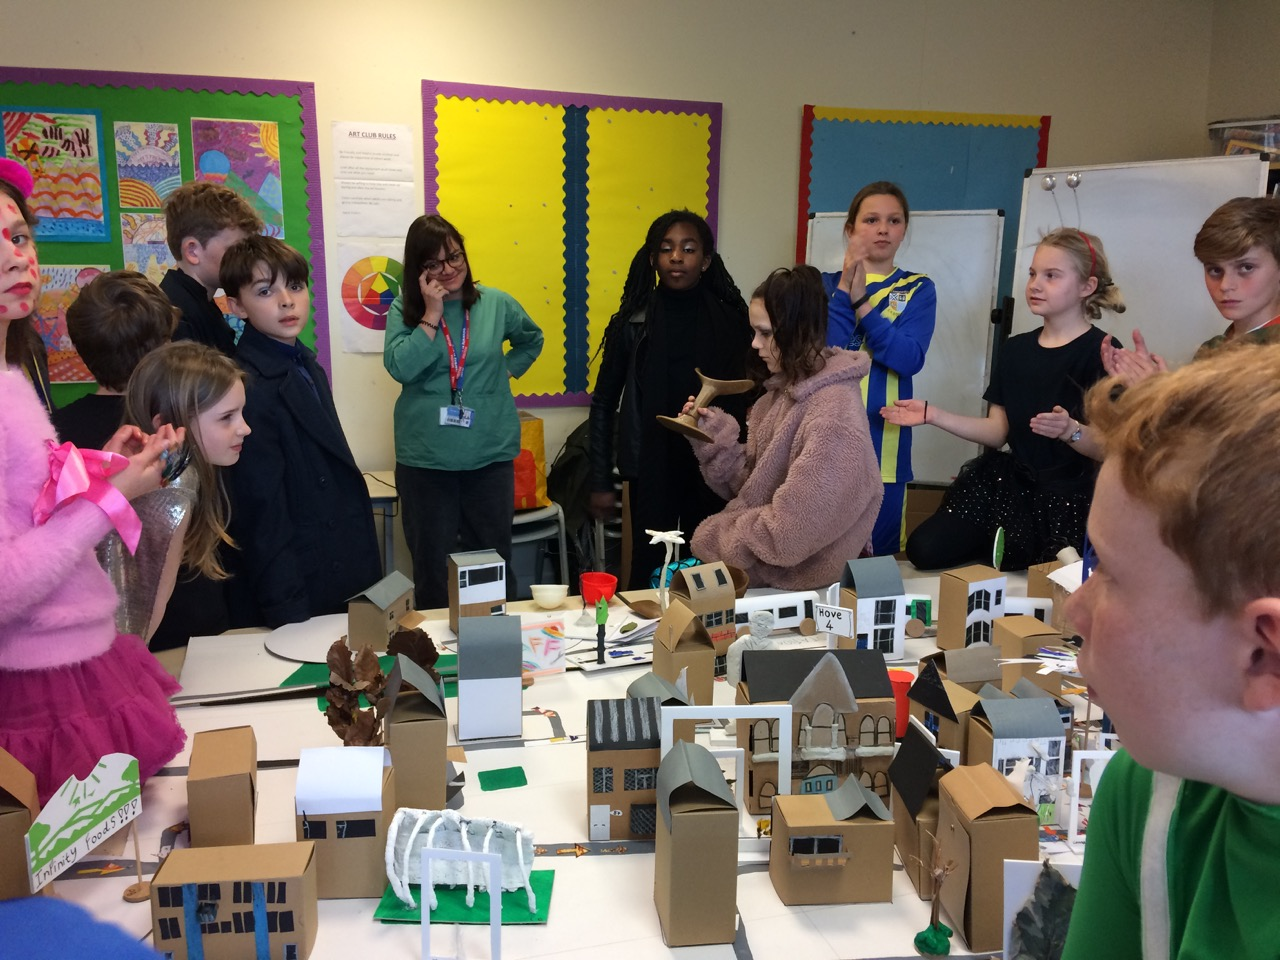
\includegraphics[width=0.35\linewidth]{images/IMG_7377}}
  \hspace{0.5in}
  \subcaptionbox{Puzzle-pot from Rez\'e Museum (France), photo courtesy of Theophane Nicola}
  {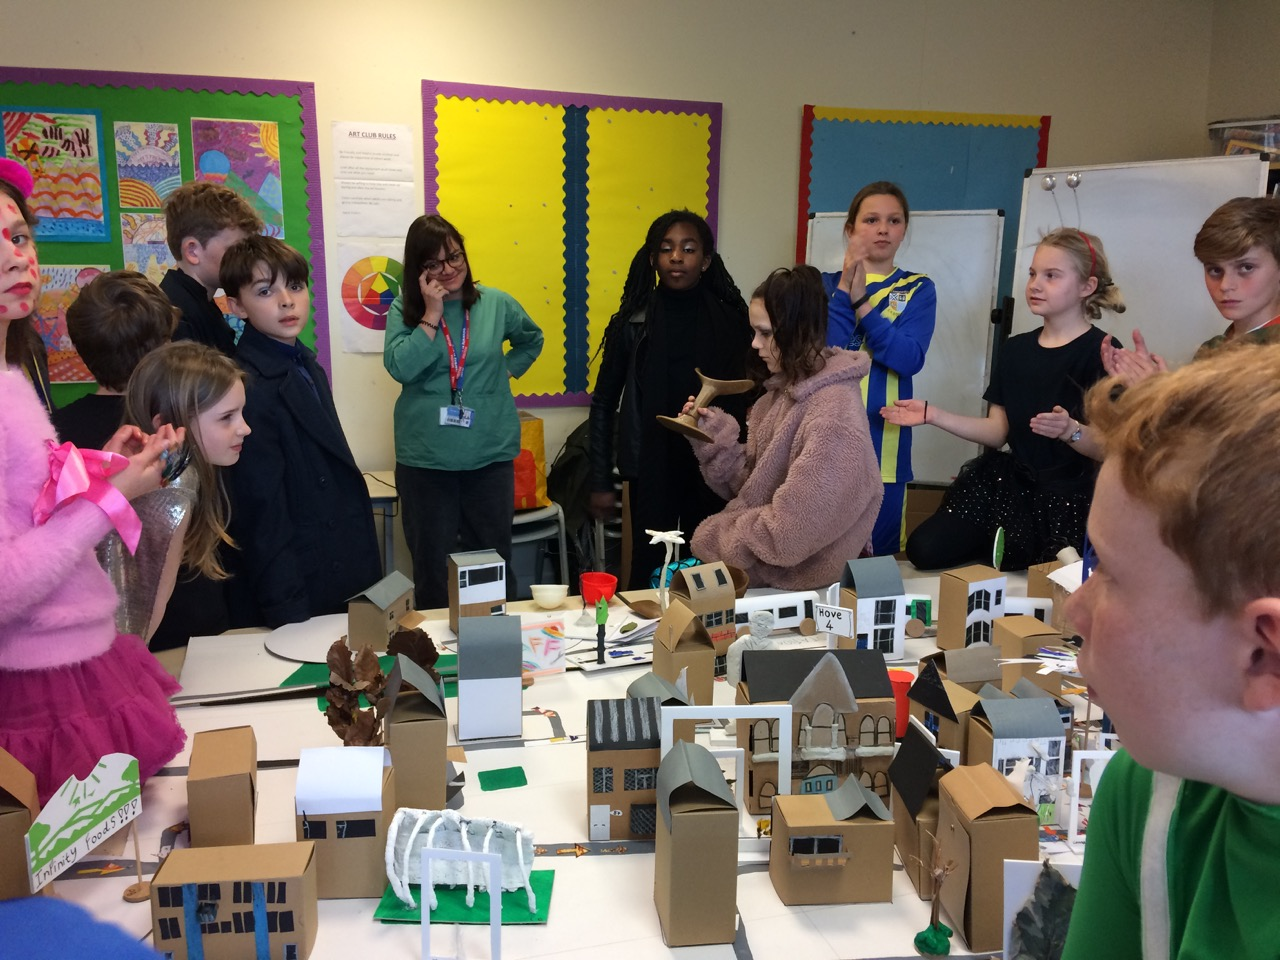
\includegraphics[width=0.35\linewidth]{images/IMG_7377}}
  \caption{\label{fig:puz}Examples of pottery puzzles in museums.}
\end{figure}

Until now, communities have rarely had an input into which heritage to preserve.
Their participation in this process might provide new insights into which
heritage is important for their community. Computer graphics technologies also
have an important role to play in this process, but limited research has
been done in this area. The research presented in this paper aims to address
this gap. In particular, it explores how entry barriers can be lowered for a
wider set of audiences to connect with their local heritage outside museum
settings. For this, it proposes the use of creative and narrative-based
approaches, given the potential for stories to illuminate different viewpoints
regarding Cultural Heritage assets. Hence, the term \textit{place-based
narratives} is used to refer to the interpretative stories linked to the
people, objects, sites and events in the urban landscape as told by the
community. As such, the research acknowledges the important relationships
between a community and the areas in which they move on a daily basis, which
can greatly enhance the public's understanding and appreciation of objects and
sites. 

The contribution of the research is twofold, firstly by proposing an approach for
the development of place-based narratives through community involvement; and
secondly by deploying novel technologies which can re-tell the
narratives. The technical contribution combines both digital technologies and
physical printed material. In this research, this development is referred to
as an \emph{Augmented Reality (AR)} Map. This is defined as a physical printed
map, such as a map of a geographical area or a building, with embedded
augmented digital 3D scenes in order to provide additional layers of
information to the user. The technology has been developed using an
\emph{Immersive Web} approach to ensure wider accessibility of the content.

The \emph{Augmented Reality (AR) Map} concept is proposed to appeal to the
user's curiosity and add further layers of understanding to the Cultural
Heritage material. It is hypothesised that this approach is of interest to the
community both in terms of user engagement and with regards to the information
transmitted. By using their mobile devices, users can trigger additional
information without being distracted from the main information conveyed by the
map. Interaction with the digital 3D scenes embedded in the map might include
the ability to visualise and interact with the narratives of communities
recorded as a mixture of content including text, images and 3D content. 

By encoding the narratives as a digital element of the experience, these
narratives can have a life of their own, evolve to take into account other
viewpoints and survive the lifespan of the physical element. Moreover, the
printed element can also serve as a physical memento of an experience, such as
a visit to a neighbourhood. In this way, the research conceptualises a
transmedia storytelling based interpretative framework for cultural heritage.
This idea can be extended to enrich cities or artefacts in museums with
multiple interpretative narratives.

The approach for creating and re-telling place-based narratives has been
deployed with a community of school children in the city of Brighton and Hove
in the UK. The children engaged through an artistic process to generate
place-based narratives of their daily journeys between home and school.
Thereafter, the narratives were converted into an AR Map.

The paper is organised as follows: Section~\ref{ref} presents related work in
this area, Section~\ref{meth} presents the methodology used in this research
to facilitate the creation of narratives by the community, while
Section~\ref{tech} describes the technology developed for the Augmented
Reality (AR) Maps. Section~\ref{eval} discusses preliminary evaluation of this
research, and finally Section~\ref{conc} presents conclusions and further
work.


\section{Related work} \label{ref} Related research on community engagement
with heritage includes the framework proposed by G{\"o}ttler and Ripp
\cite{icomos1812}, which formulate different levels of community engagement
with built heritage assets, including awareness, exploration, participation
and transfer. It proposes the use of digital communication technologies to
enable a multi-directional communication between heritage organisations and
communities. This communication can be underpinned by a variety of engagement
initiatives and a mixture of digital content, including stories, photographs
and geographical information. Other approaches have demonstrated how
communities can be engaged in creative process for co-designing artworks
\cite{656aab9e240d4479bf2872665a590233}, and other digital experiences of
heritage \cite{ Avram:2019:CGL:3358680.3348793, Fox:2014:CHS:2598510.2598563,
Albouys-Perrois:2018:TMA:3173574.3174203}. 

There has also been previous interest in combining AR with printed material,
for example in children's books which contain a QR code for displaying AR
content. Moreover, physical maps have been proposed as backgrounds for
embedding digital content which relate to the geographical location, such as
photos, video and their metadata \cite{Morrison:2009:LBA:1518701.1518991,
Terracciano:2017:MMR:3027063.3052958}.

This research advances the research agenda on community engagement with both
tangible and intangible heritage in urban space. Our emphasis is on the
development of technological solutions which enable the incorporation of multiple
views and perspectives, including those of experts and non-experts. For this,
the following section will  describe methods for engagement which are
accessible to a variety of audiences, followed by digital technologies for
documenting and re-telling these experiences. 


%-------------------------------------------------------------------------
\section{Methodology for engaging communities with their CH through place
based narratives} 
\label{meth} The methodology of the research was designed by
a multi-disciplinary team of experts including Cultural Heritage (CH)
professionals, members of a civic group, education specialists, artists,
well-being professionals and computer scientists. In the initial stage, the
research focused on children as it is possible to engage with them through
formal education. In particular, the research engaged with children between
the ages of 10-11 studying at a local primary school, in the year before they
move to secondary school.

Figure~\ref{fig:method} illustrates the methodology for conducting the
research, which includes the following stages: design of the experience,
creative development of narratives, capturing narratives through digital
technology, wider engagement with the community and evaluation.


\begin{figure}[b]
  \centering
  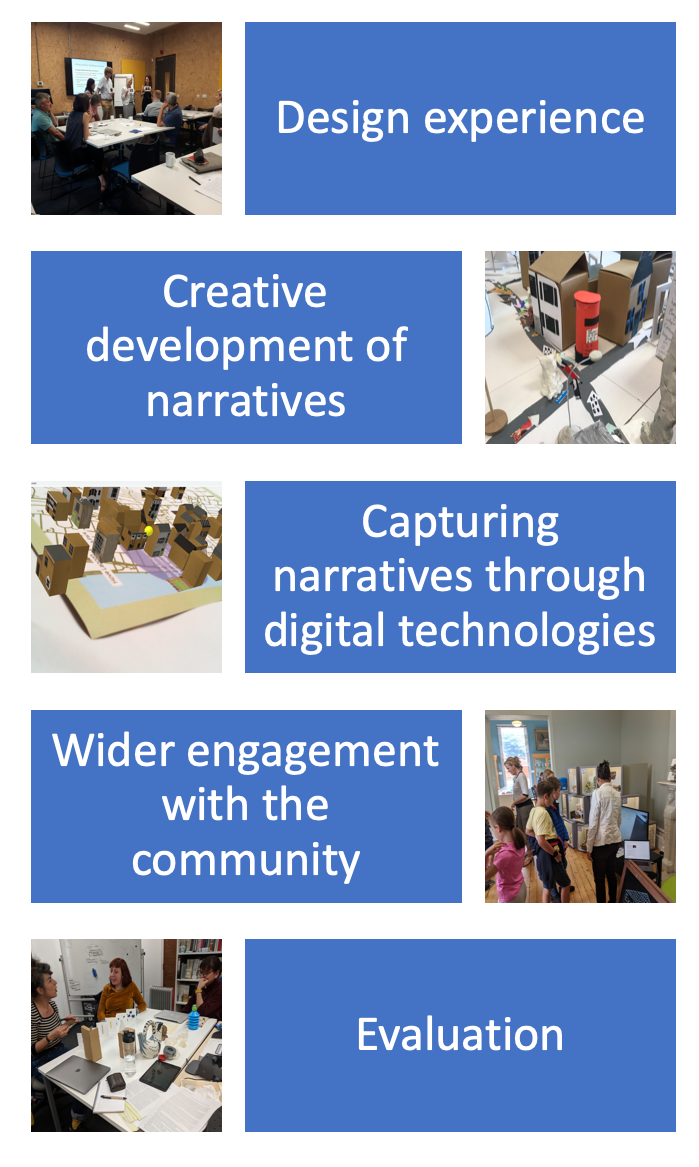
\includegraphics[width=0.6\linewidth]{images/method}
  \caption{\label{fig:pot}
    Late Iron Age funerary urn from Saltdean, Sussex (UK).}
\end{figure}

% \begin{figure}[b]
%   \centering
% 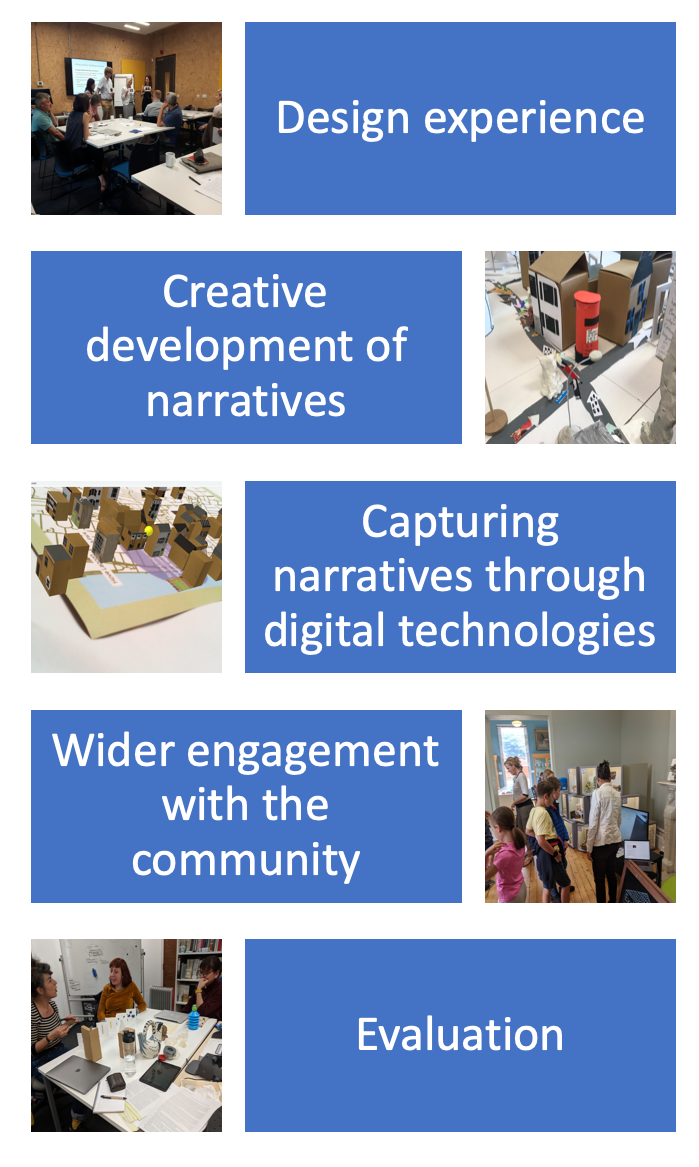
\includegraphics[width=0.8\linewidth]{images/method.png}
% \caption{Methodology for engaging with communities deployed by the research}
% \label{fig:method} 
% \end{figure}

During the design of the experience, the team aimed to understand how children
could engage with their cultural environment while addressing subjects in the
curriculum, stimulating their creativity and addressing their well-being
needs. Particular attention was placed on identifying any particular issues
concerning the children who will be involved in the experience, including any
educational or well-being issues that they might be experiencing at that point
in time. These issues are context dependent and are likely to be affected by
external factors including community cohesion, socio-economic situation and
pressures from friends and family.

Thereafter, an artist facilitated ten workshops at the school in order to
enable children to create narratives. These workshops used creative methods
and psycho-geography techniques to explore the journeys children make from home
to school five days a week. Psycho-geography refers to the study of the effects
of the geographical environment on the emotions and behaviours of individuals
\cite{coverley2006psychogeography}. 

The focus on the daily home-school journey was chosen due to the fact that
these journeys are a practical everyday routine. It is common that people
don't pay much attention to the places, objects and details they pass along
the route. As such, the workshops facilitated the exploration of a series of
questions:

\begin{itemize} 
  \item How do the children feel about travelling the same route five days a week, every week?   
  \item How much are children aware of the physical environment around them on these journeys? 
  \item Where do children look when they walk? 
  \item What do children daydream about? 
\end{itemize}

As a result, children were encouraged to look up, down and all around their
local environment. They were encouraged to try to look at the streets where
they walk in a different way. In doing so, children became historians,
journalists, archaeologists in reverse, creative observers of everyday life.
Narratives, both of the children's personal lives and of elements in the
geographical landscape, were created as a result of this process. These
\emph{place-based narratives} used a mixture of physical, visual and textual
material. 

There was no involvement of digital technologies at this stage, as it was
decided children could explore more freely their environment without the
mediation of a digital device. Instead, each child produced a decorated box
which represented their house as illustrated by Figure~\ref{fig:boxes}. This
was the first observation task as many children had not, until that point,
really paid attention to the fa\c{c}ade of their houses. Boxes were used both
as markers and containers of the child's personal narrative. There were no
limitations on what material children could use to capture their narratives.
As a result, crafted elements were created from a mixture of materials such as
clay, cardboard, foam, plastic, wire, foliage, feathers.
Figure~\ref{fig:artwork}-left illustrates a mixture of the crafted material
which was produced. Children also produced drawings or collages using a
mixture of material (e.g. foliage, printed images), illustrating their
journeys (see example Figure~\ref{fig:drawingmaps}). Some children wrote
textual content with stories of people, objects, sites and events they
researched on. 

Finally, all elements were organised according to their geographical location
on a physical 3D map. This crafted artwork piece celebrates the individual
interpretative narratives and the collective journeys made by the children all
converging at the shared community of school (see Figure~\ref{fig:artwork}). 

\begin{figure}[ht] \centering
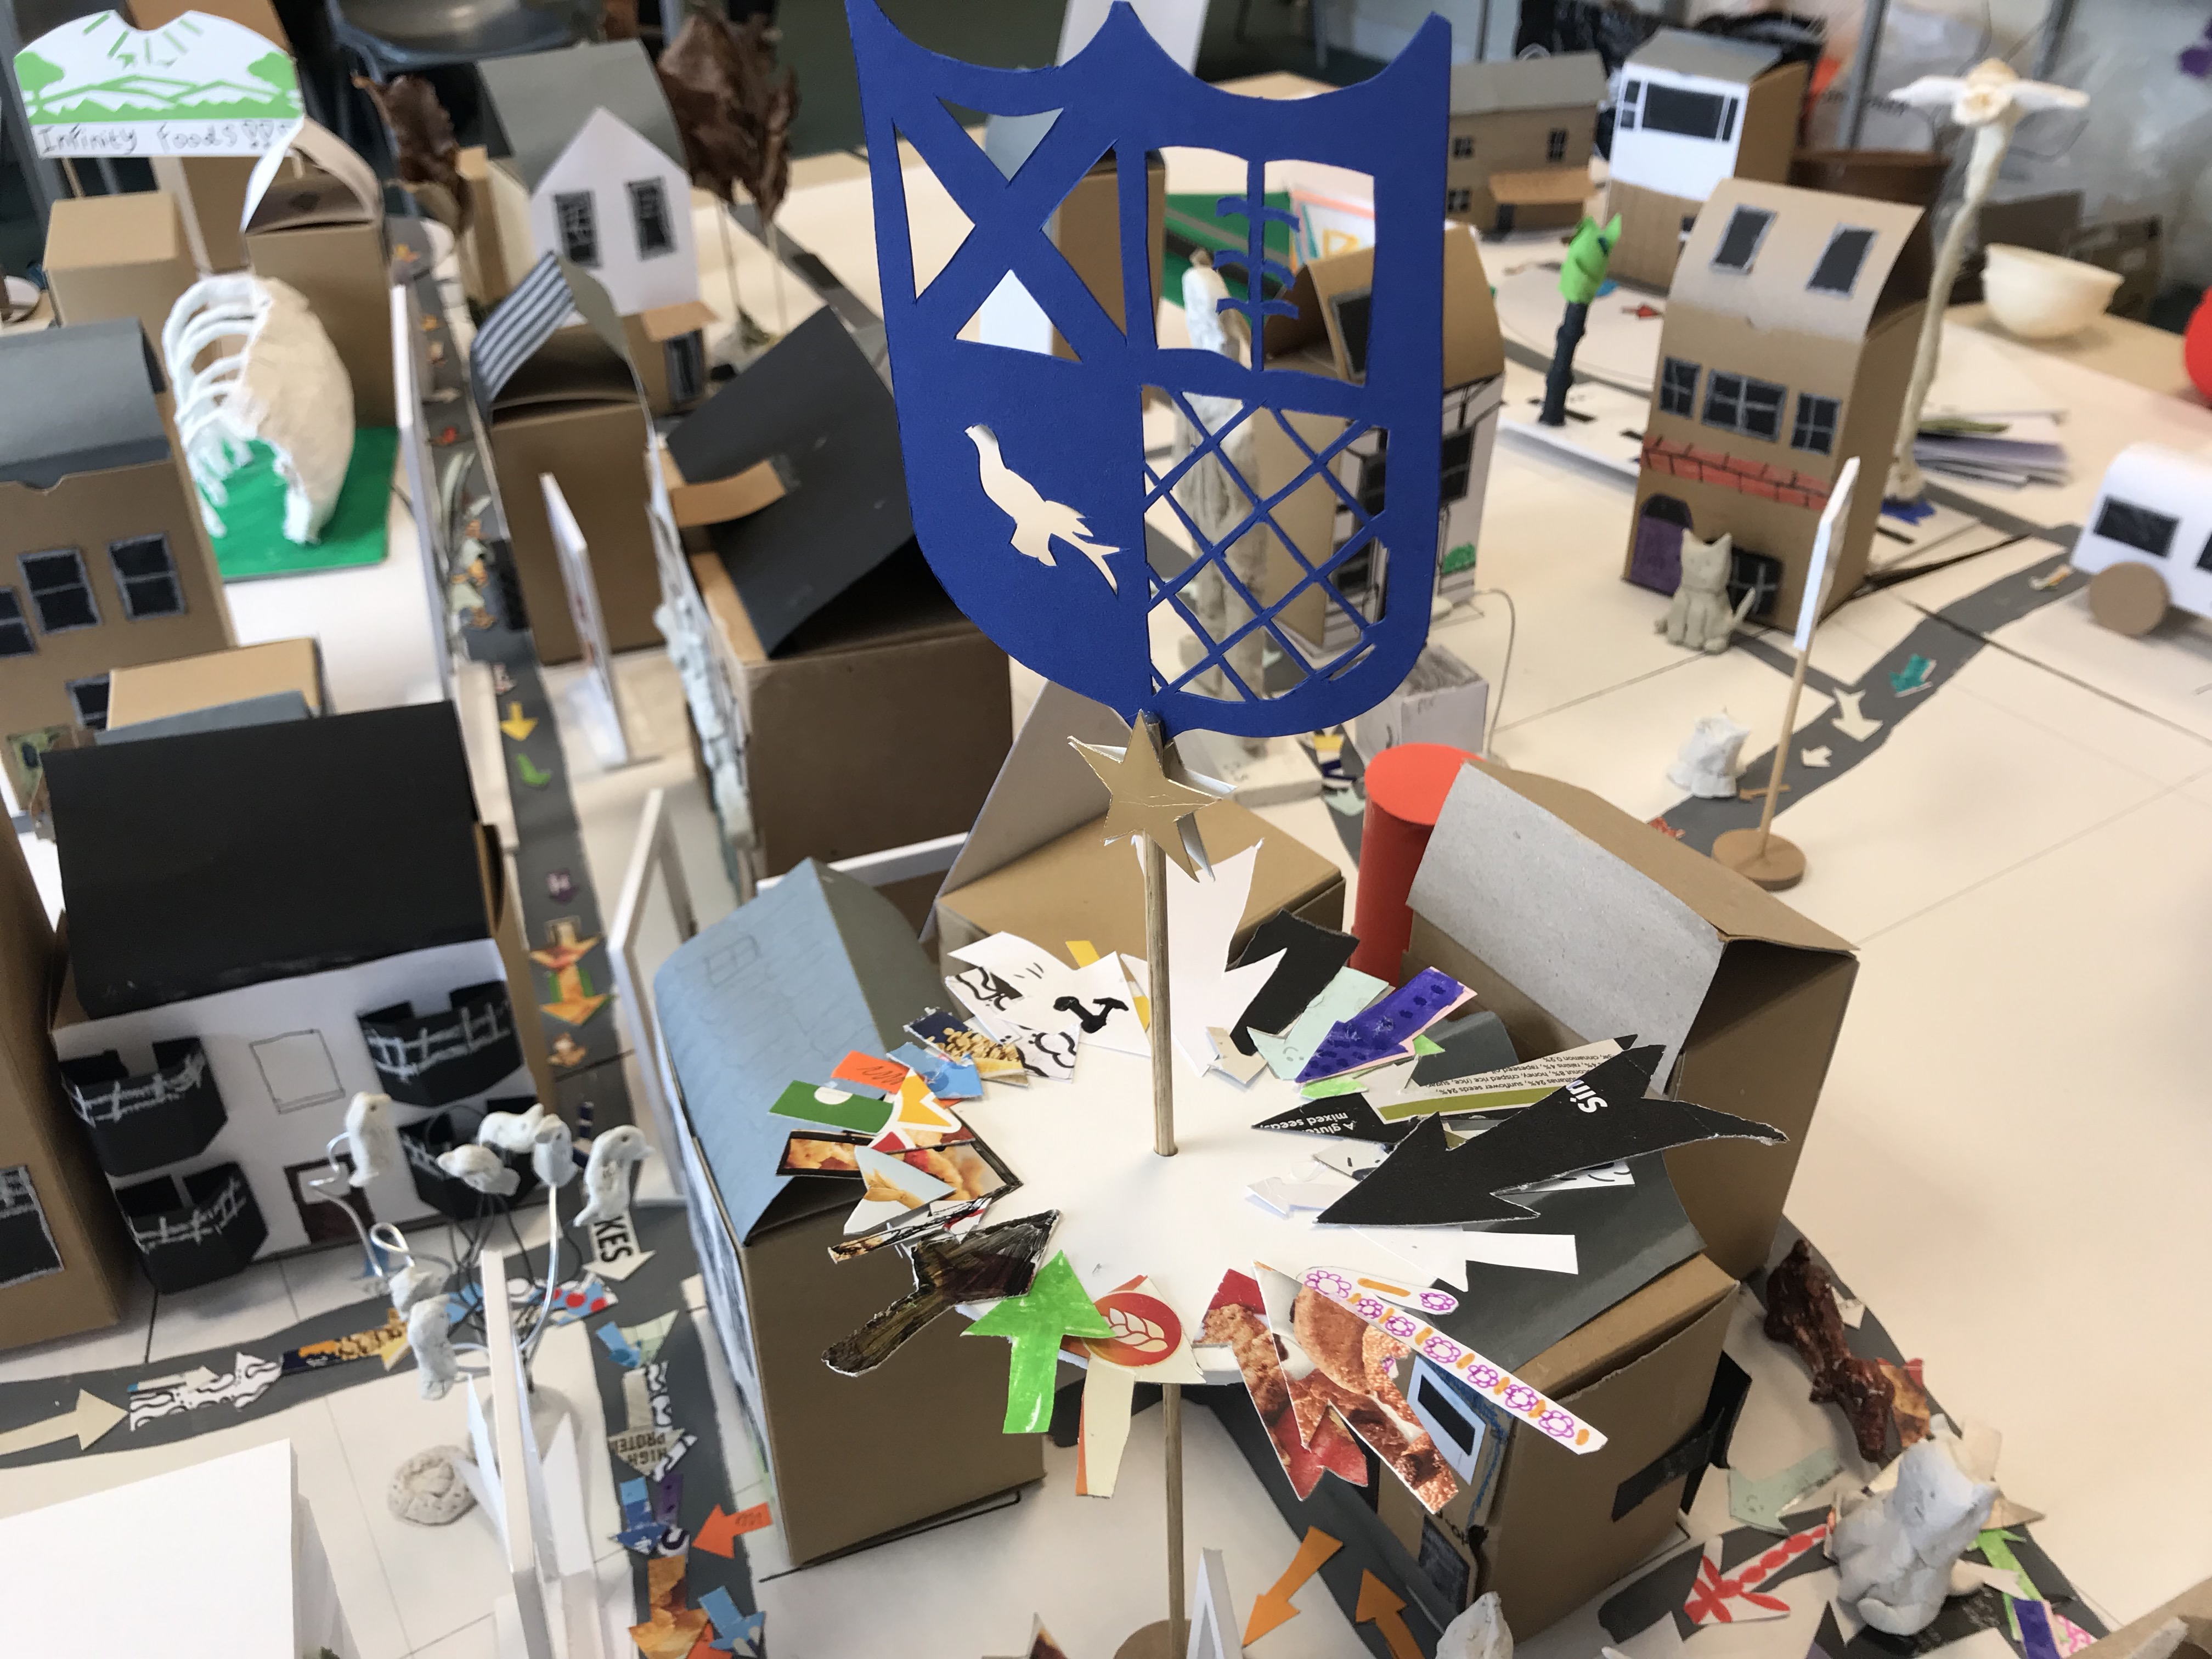
\includegraphics[width=\linewidth]{images/variousassets.jpg}
\caption{Crafted objects produced during the workshops documenting place-based
narratives} \label{fig:artwork} \end{figure}

The next steps in the methodology are explained in the following sections.

% \textbf{\begin{figure}[ht] % %     \centering % %    
% 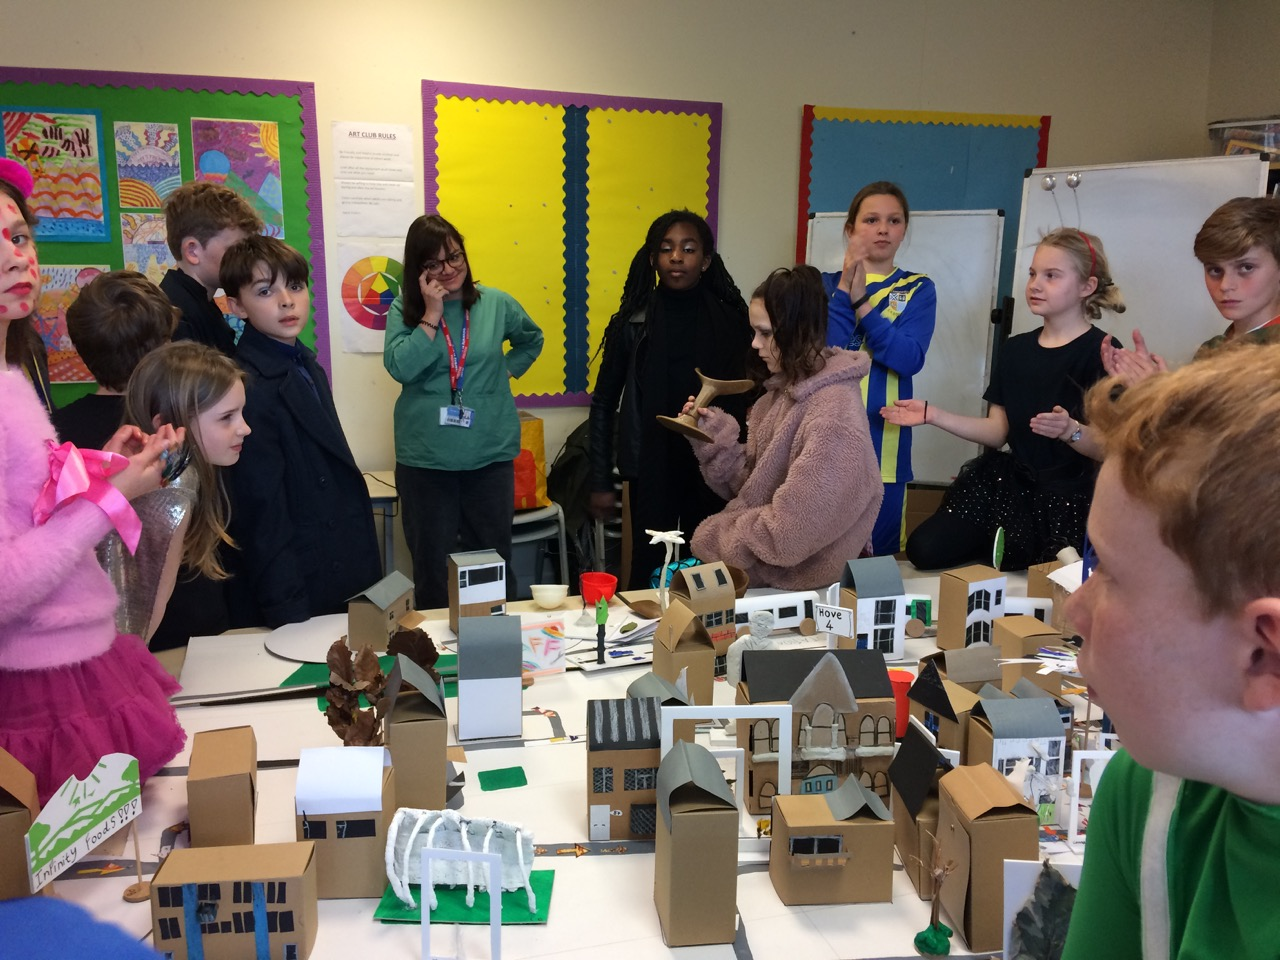
\includegraphics[width=\linewidth]{images/IMG_7377.jpeg} % %     
% \caption{Children with artwork documenting place-based narratives of central
% Hove} 
% \label{fig:childart} 
% \end{figure}} %
%-------------------------------------------------------------------------
\section{Augmented Reality (AR) Map Development} \label{tech} Normally, the
outcomes of psycho-geography and participatory approaches, which are not
mediated by technologies, are lost shortly after the process of engaging with
communities. The reason is that, as demonstrated by the resulting crafted
objects (Figure~\ref{fig:artwork}), while the materials which are used  are
amenable to creative approaches they are not necessarily easy for
digitisation. Hence, results from these participatory approaches are normally
disposed of shortly after their display and are rarely disseminated to
 a larger audience in their original form. 

This research explored the role of graphics technologies for i) the
digitisation of the narratives produced in order to support their
documentation and preservation; and ii) re-telling these narratives to others.
These audiences include other members of the same community, audiences who are
new to the geographical area and other stakeholders who might have an interest
in better understanding which elements of the cultural landscape are
significant to the community.

While the process for digitisation is better understood by the research
community - in terms of deciding which technologies to use for which artefacts
- the requirement to re-tell the narratives has not previously been fully
explored. Thus, there are many potential digital experiences which could be
used for this purpose. 

A novel approach for re-telling these narratives is proposed. This approach
combines elements of a physical and a digital experience. The digital element
is intended to serve as a canvas for users to interact with the journeys and
find more information relevant to the narratives through hyperlinks. 

From early on in the research, it was clear that communicating the
geographical location was critical to re-telling the narratives. However,
using precise geographical information, such as in a Geographical Information
System (GIS), was not possible without having to reveal the exact location of
the address of members of the community. Hence, the idea of providing the
content geographically in-situ was discarded. Instead, the research
incorporated an experience very familiar to people when visiting a new
location. This is the communication of specific information through a printed
map (e.g. a tourist map or a building map). Printed maps allow the
abstraction of geographical/spatial information while enabling the reader to
orient themselves in the space. Augmented Reality (AR) is then used to embed
the digitised narratives without losing their geographical information. AR
also has the advantage that multiple interpretations can be embedded in
parallel to the same visual information. 

The research also considered the need to create physical media which is
cost-effective to produce and distribute to a large audience. As such, all
physical elements of the experience can easily be reproduced by the user by
printing a PDF map. Moreover, the digital element is easily accessible from a
web browser on a PC, tablet or smartphone so that there is no need to install
. 

The Augmented Reality web-application renders a 3D scene with the crafted
houses, which are positioned over the printed map in a similar way to the
crafted artwork (see Figure~\ref{fig:ARexperience}). When the user clicks or
taps on each of the houses, an animation is triggered to simulate the box
being opened. The content inside the box is then rendered on a viewer for the
viewer to inspect in more detail. 

The following sub-sections will describe in detail how the different
components of the Augmented Reality (AR) map were developed.

\subsection{Development of printed graphical map} %talk about the development
process for the printed map: mapnik, openstreetmap data, rendering of scene, 
The development of a printed map addressed various requirements as described
below:

\begin{itemize} 
  \item Display information on the street layout in a way which is easy for the user to understand. 
  \item Not reveal the precise geographical location of the houses. 
  \item Be self-contained in terms of telling the user how to access 
  the digital element of the experience. 
  \item Include a marker for the Augmented Reality which is not too distracting. 
\end{itemize}

In order to address the first two requirements, a customised rendering of a
map was created. This map displayed information, which is geographically
accurate, but detailed information, such as street names, were omitted. The
open-source mapping toolkit Mapnik \cite{mapnik} was used to generate the map.
This toolkit, with binding in Python, can programmatically generate rendering
of geographical maps with the appearance the user wants. For this, an XML
stylesheet is created which filters only the information of the streets for
rendering and provides other information such as colour and line thickness.
Thereafter, a Python script processed this stylesheet to produce the final
rendering. Geographical data of Brighton and Hove (UK) was retrieved from OpenStreetMap
\cite{OpenStreetMap} in the OSM data format. This data was then used as input
to the script in order to produce the rendering of the map in PNG format (see
Figure~\ref{fig:map}).


\begin{figure}[b]
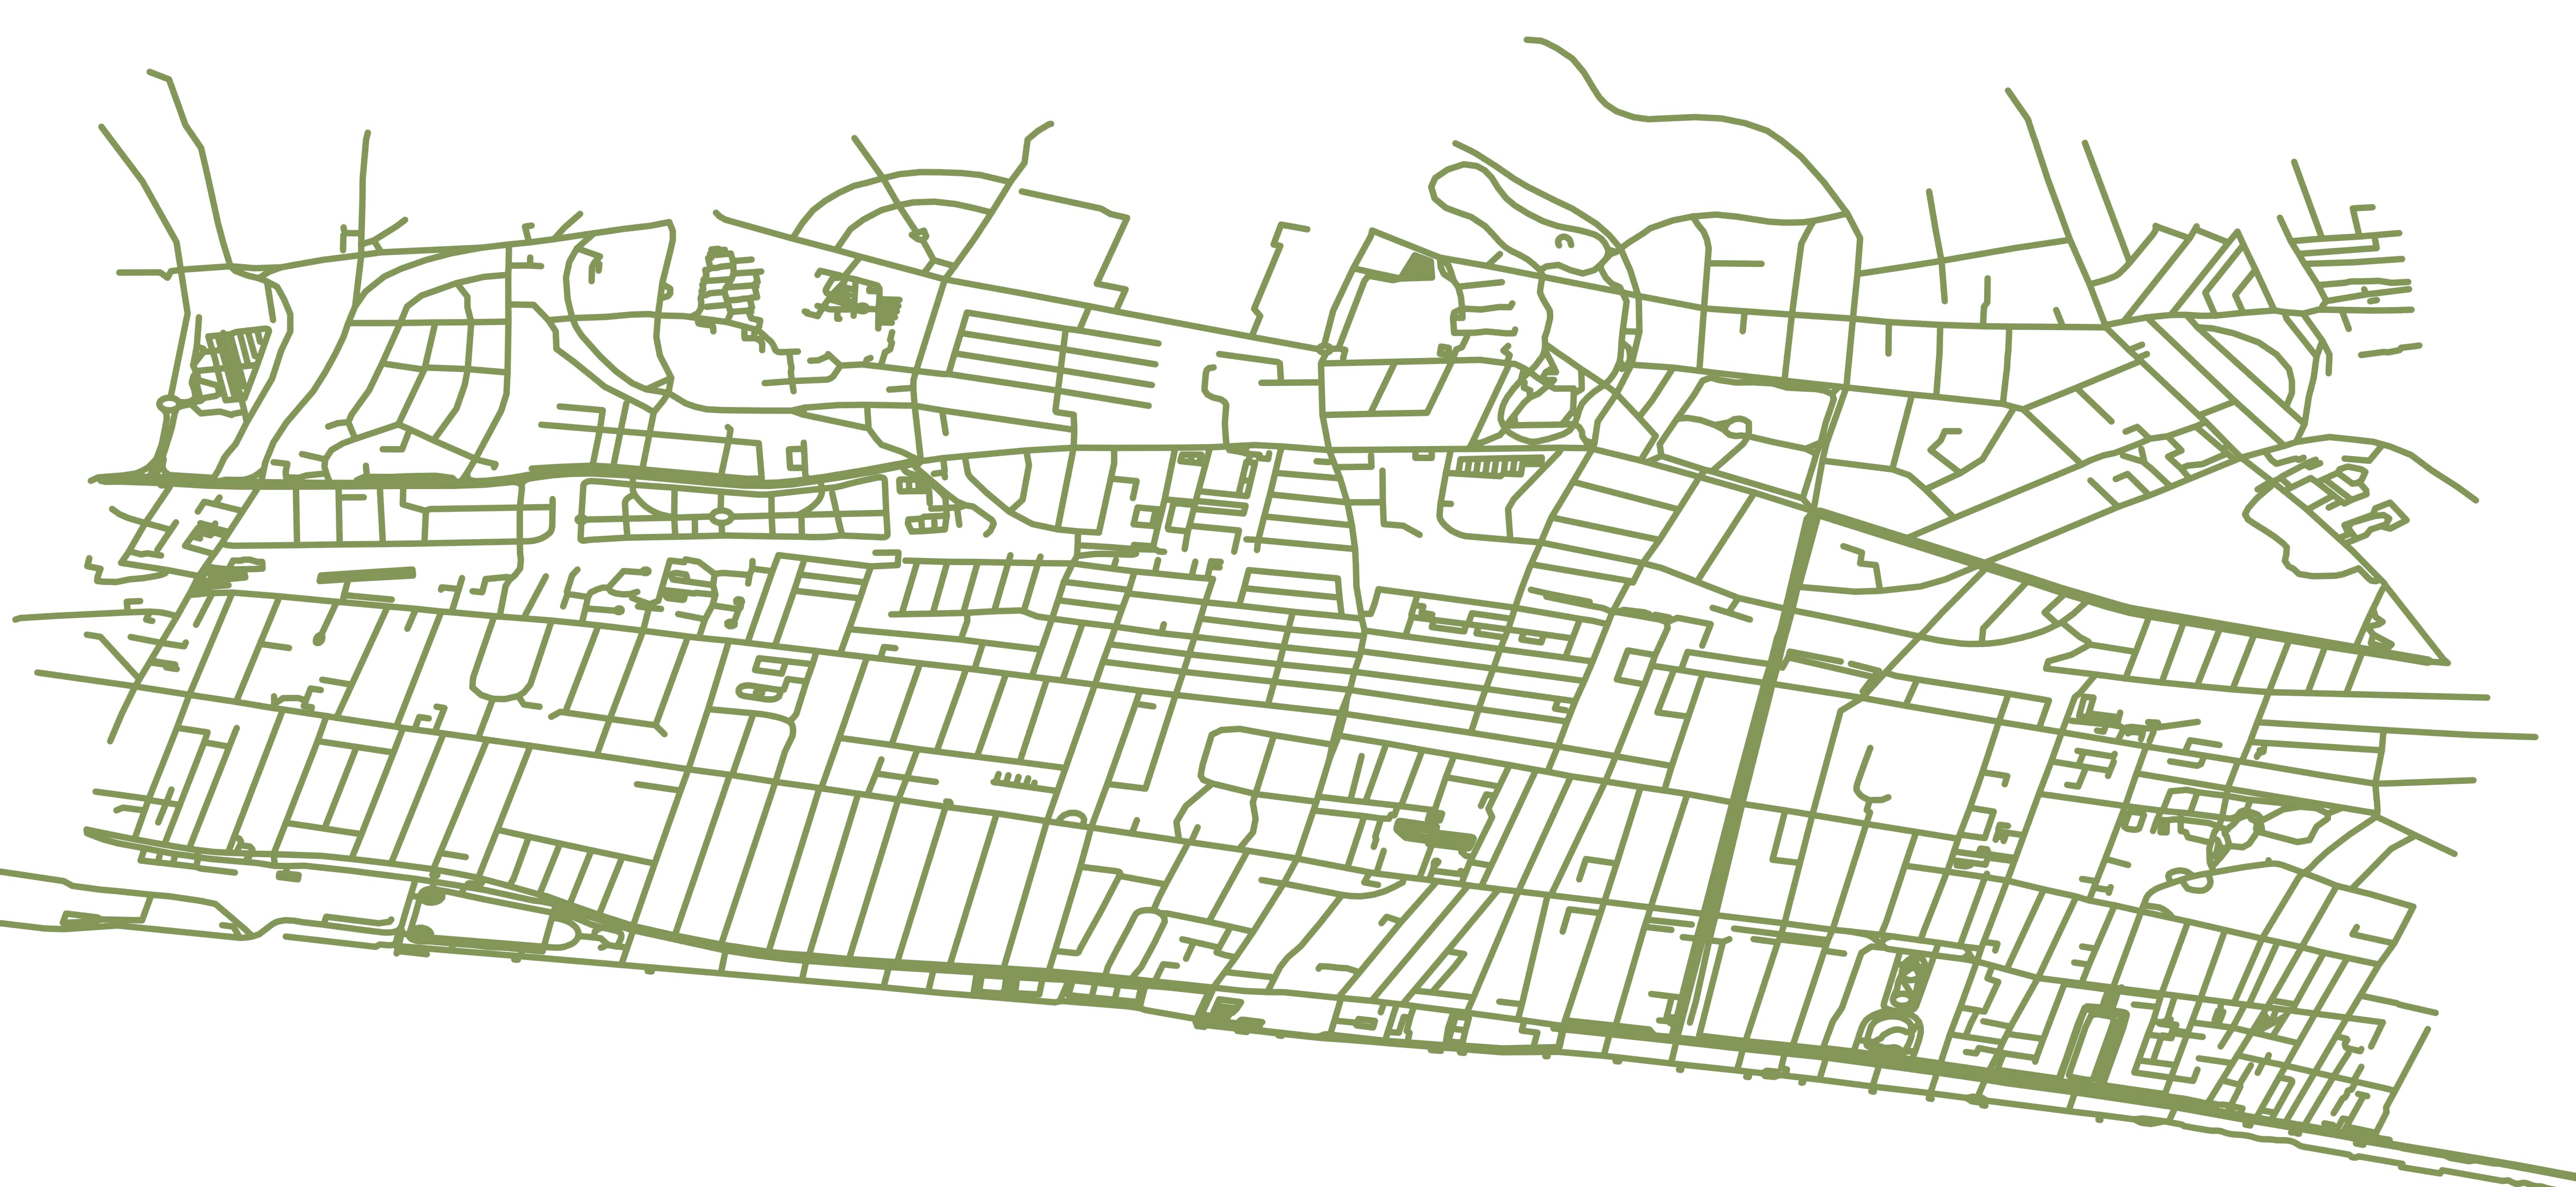
\includegraphics[width=\linewidth]{images/maprender.jpg}
\caption{Rendering of map using Mapnik toolkit} \label{fig:map} 
\end{figure}
 
The rendering of the map was further processed in the GIMP image processing
tool \cite{gimp} to include as additional information the names of relevant
geographical references. All references were extracted from the children's
narratives and included historic buildings, libraries, museums, parks,
cemetery and sculptures. Instructions on how to access the website with the AR
experience were also included.

Furthermore, a fiducial code or marker with the logo of the school was
included as illustrated in Figure~\ref{fig:print}. The marker serves both as a
way to identify the geographical location of the school as well as to enable
the AR content. Other markerless solutions were considered. However, AR over
the web does not yet have the performance required for marker-less AR, which
is normally distributed via apps and often reliant on Google's ARCore
software. Hence, not wanting to compromise in web-based delivery, the
logo-based marker was considered a suitable solution.


Finally, general information about the project was included for printing as a
double-sided page (see Figure~\ref{fig:print}). In this way, the double-sided
page is a self-containing output of the project.

% The following subsection will describe how the 3D scene which is augmented
% on the map was developed.


\subsection{Digitisation of 3D scene for AR} There were several considerations
made in order to digitise the physical artwork using 3D technologies. These
decisions were driven by the fact that the content was going to be rendered as
augmented content on the map. Hence, important requirements were to keep high
framerates as well as to include content from every child. This meant that the
houses and their content were prioritised for digitisation. Other crafted objects, 
such as those containing foliage, feathers and wire were deemed too challenging 
for their digitisation during this stage of the project.

The first task was to produce the 32 3D models of the boxes as well as to
digitise all content inside the boxes. A mixed approach was used to create the
3D models of the houses. Given the fact all houses are based on a physical box
which can be represented by a cuboid (see Figure~\ref{fig:boxes}), the use of
3D scanning or photogrammetry was discarded in favour of 3D modelling the
boxes using the modelling tool Blender\cite{blender}. 


\begin{figure}[ht] \centering
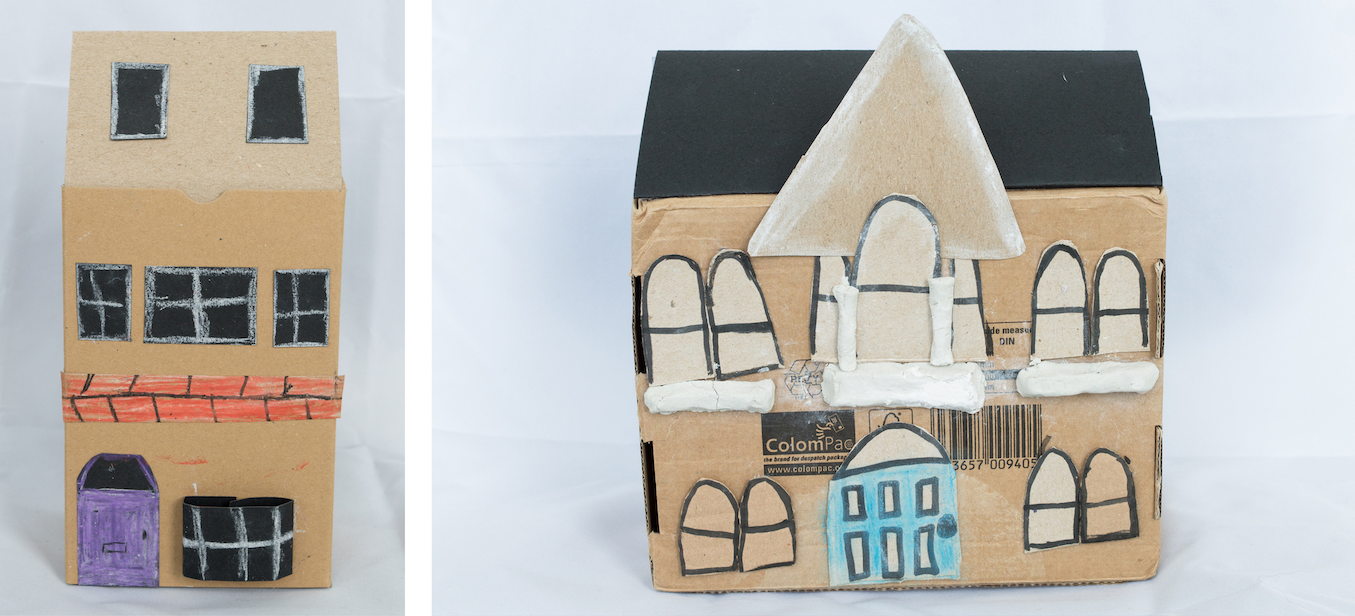
\includegraphics[width=\linewidth]{images/boxes.png} \caption{Example
of physical model houses crafted by children depicting their own houses}
\label{fig:boxes} \end{figure}

In the Blender program, simple primitives, such as cubes and planes, were used
to create the shape of each house. The geometries of the houses each began as
a simple cube, with additions such as balconies, porches or roofs being
created through the addition of planes.


The textures for each house were created from images taken with a digital
camera. The camera used was a mirrorless Sony a7R III with a Sigma 1:1.4 DG
macro lens. The houses were placed on a 360 electronic turntable, with two
Elinchrom 1000 ELC Pro HD lights with Elinchrom Rotalux softboxes used to
provide diffuse lighting. This setup ensured that the textures for each side
of the cuboid could be captured with some degree of automation while ensuring
high quality results.
 
 The number of photos required for each house depended on the geometry of the
 house. Some houses required only one image (of the fa\c{c}ade) with a simple
 cardboard texture used for all other faces, while others needed up to four
 (one for each side). Many of the houses required additional images due to
 features such as roofs or gutters. The images were taken at an angle
 perpendicular to each face in order to avoid any perspective effect. 

 \begin{figure}[ht] \centering
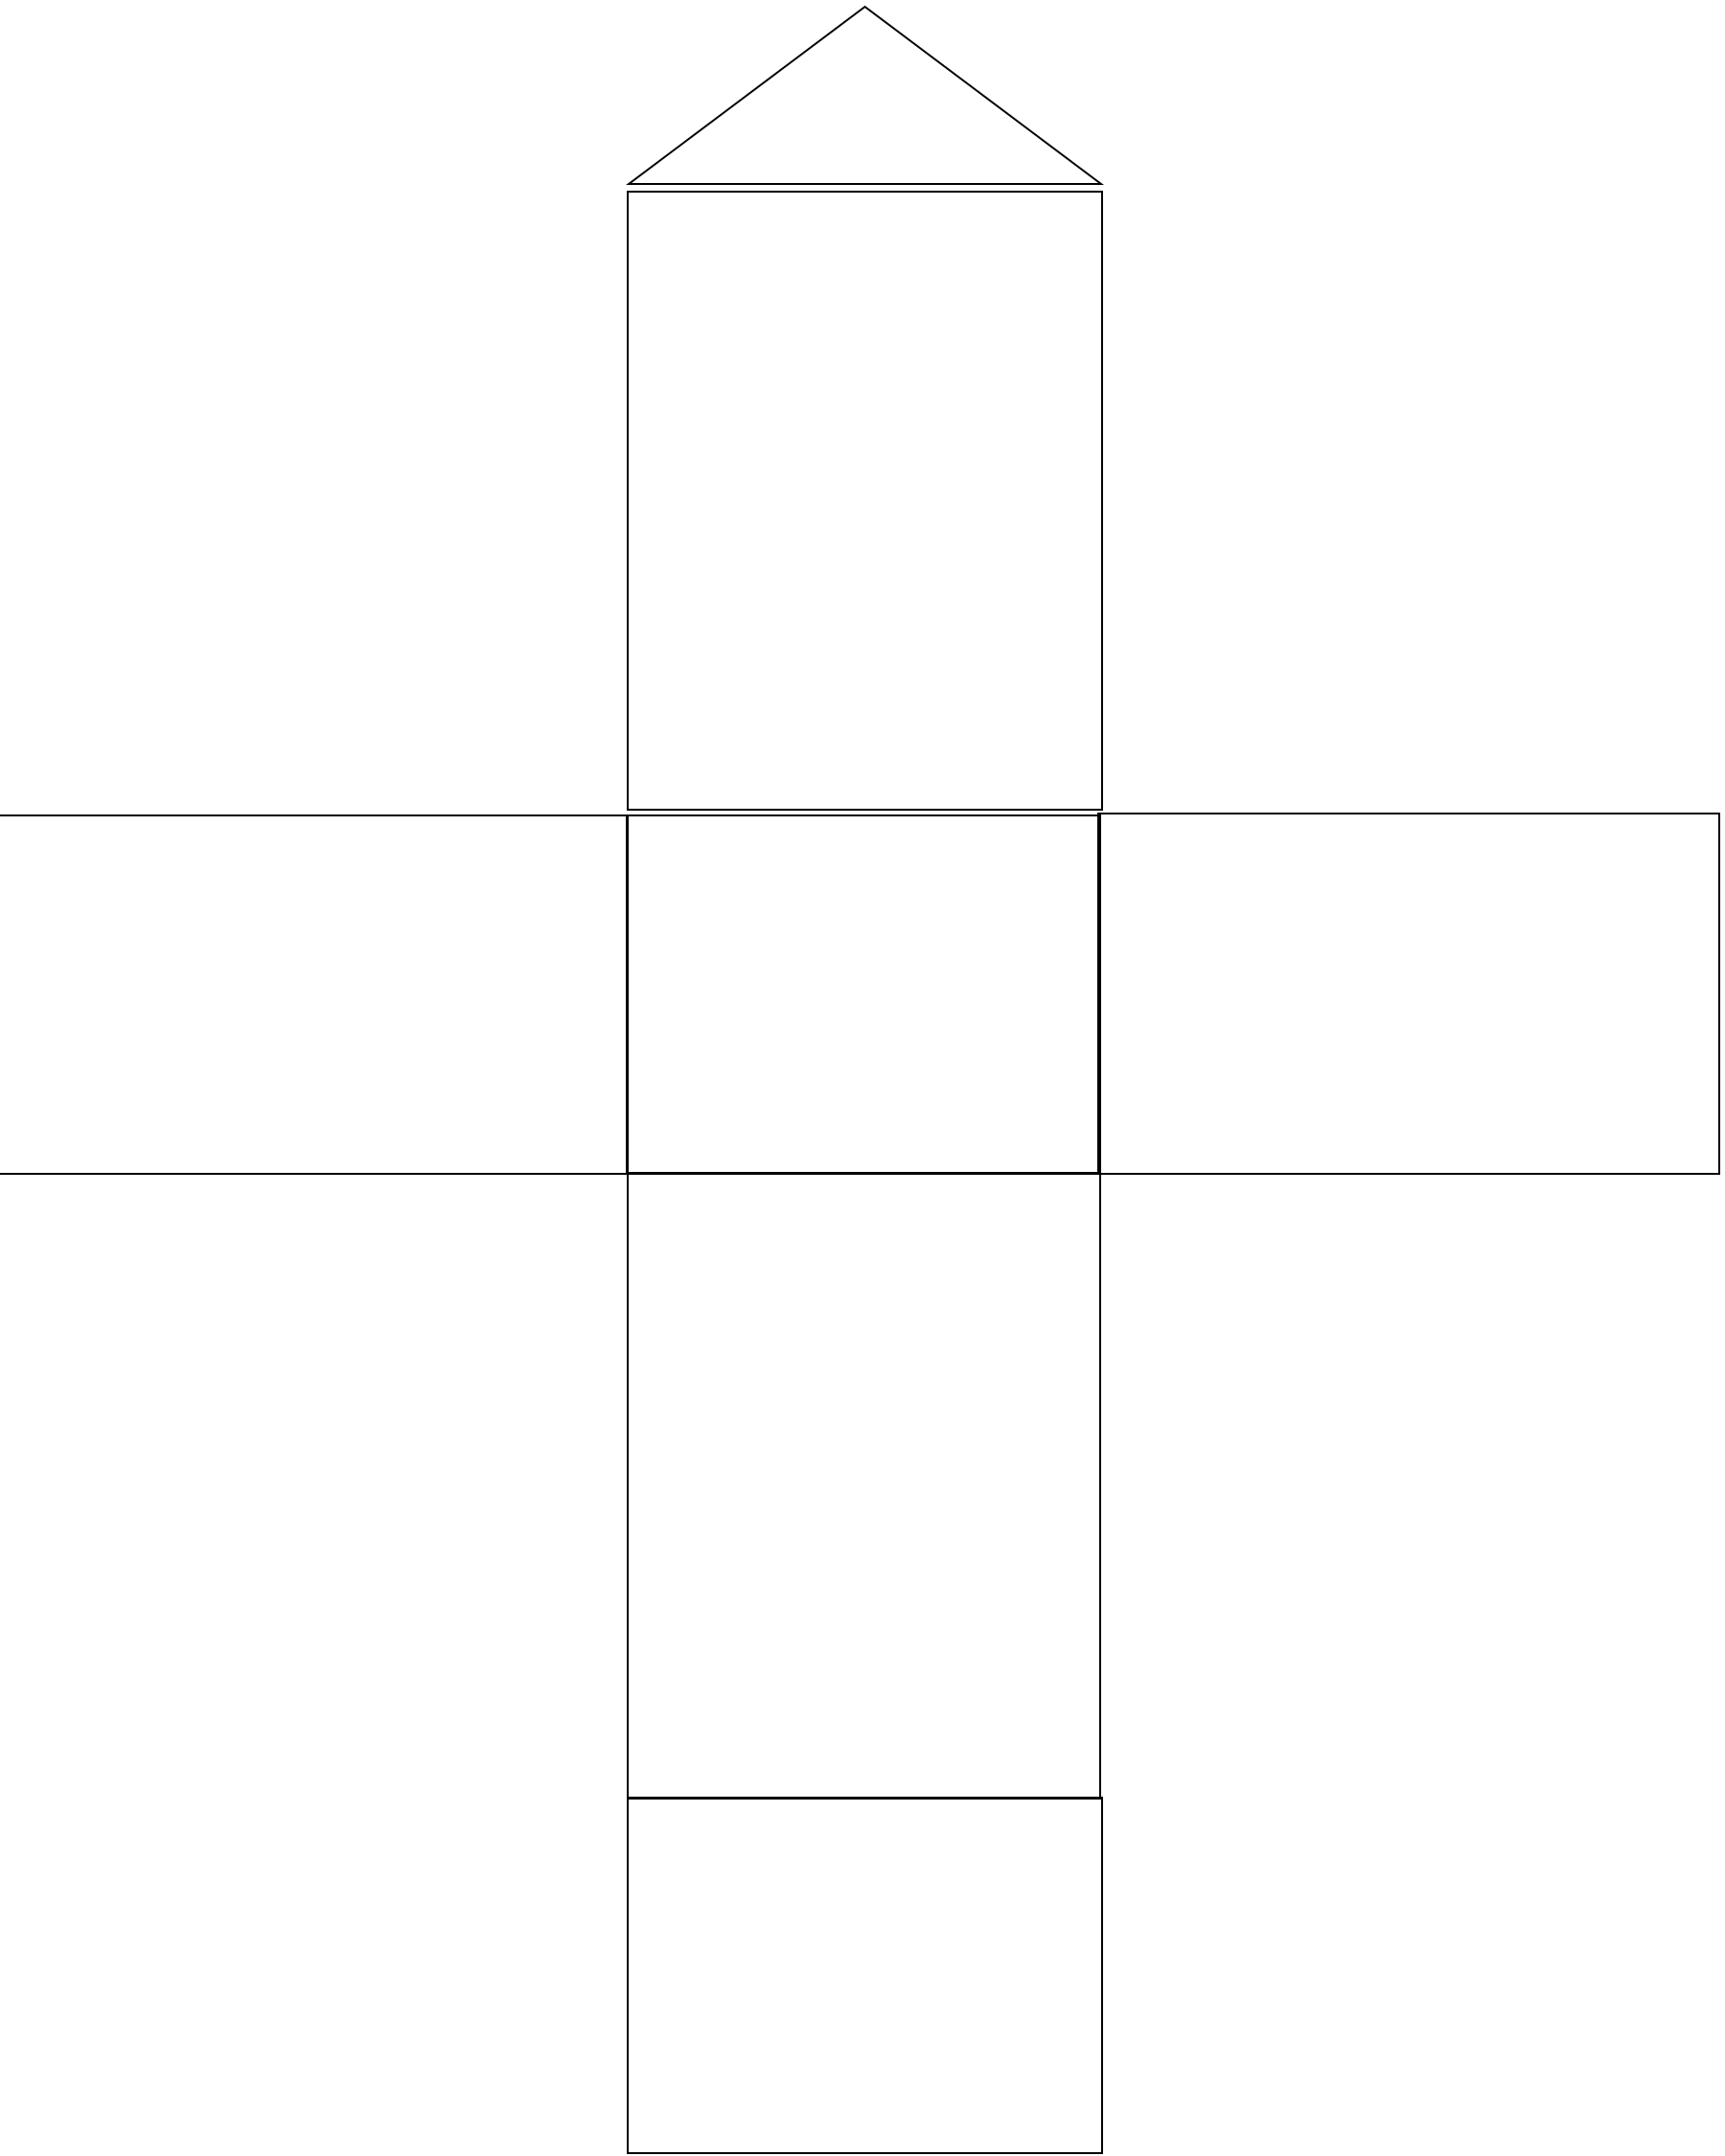
\includegraphics[width=0.49\linewidth]{images/za_tex_template.png}
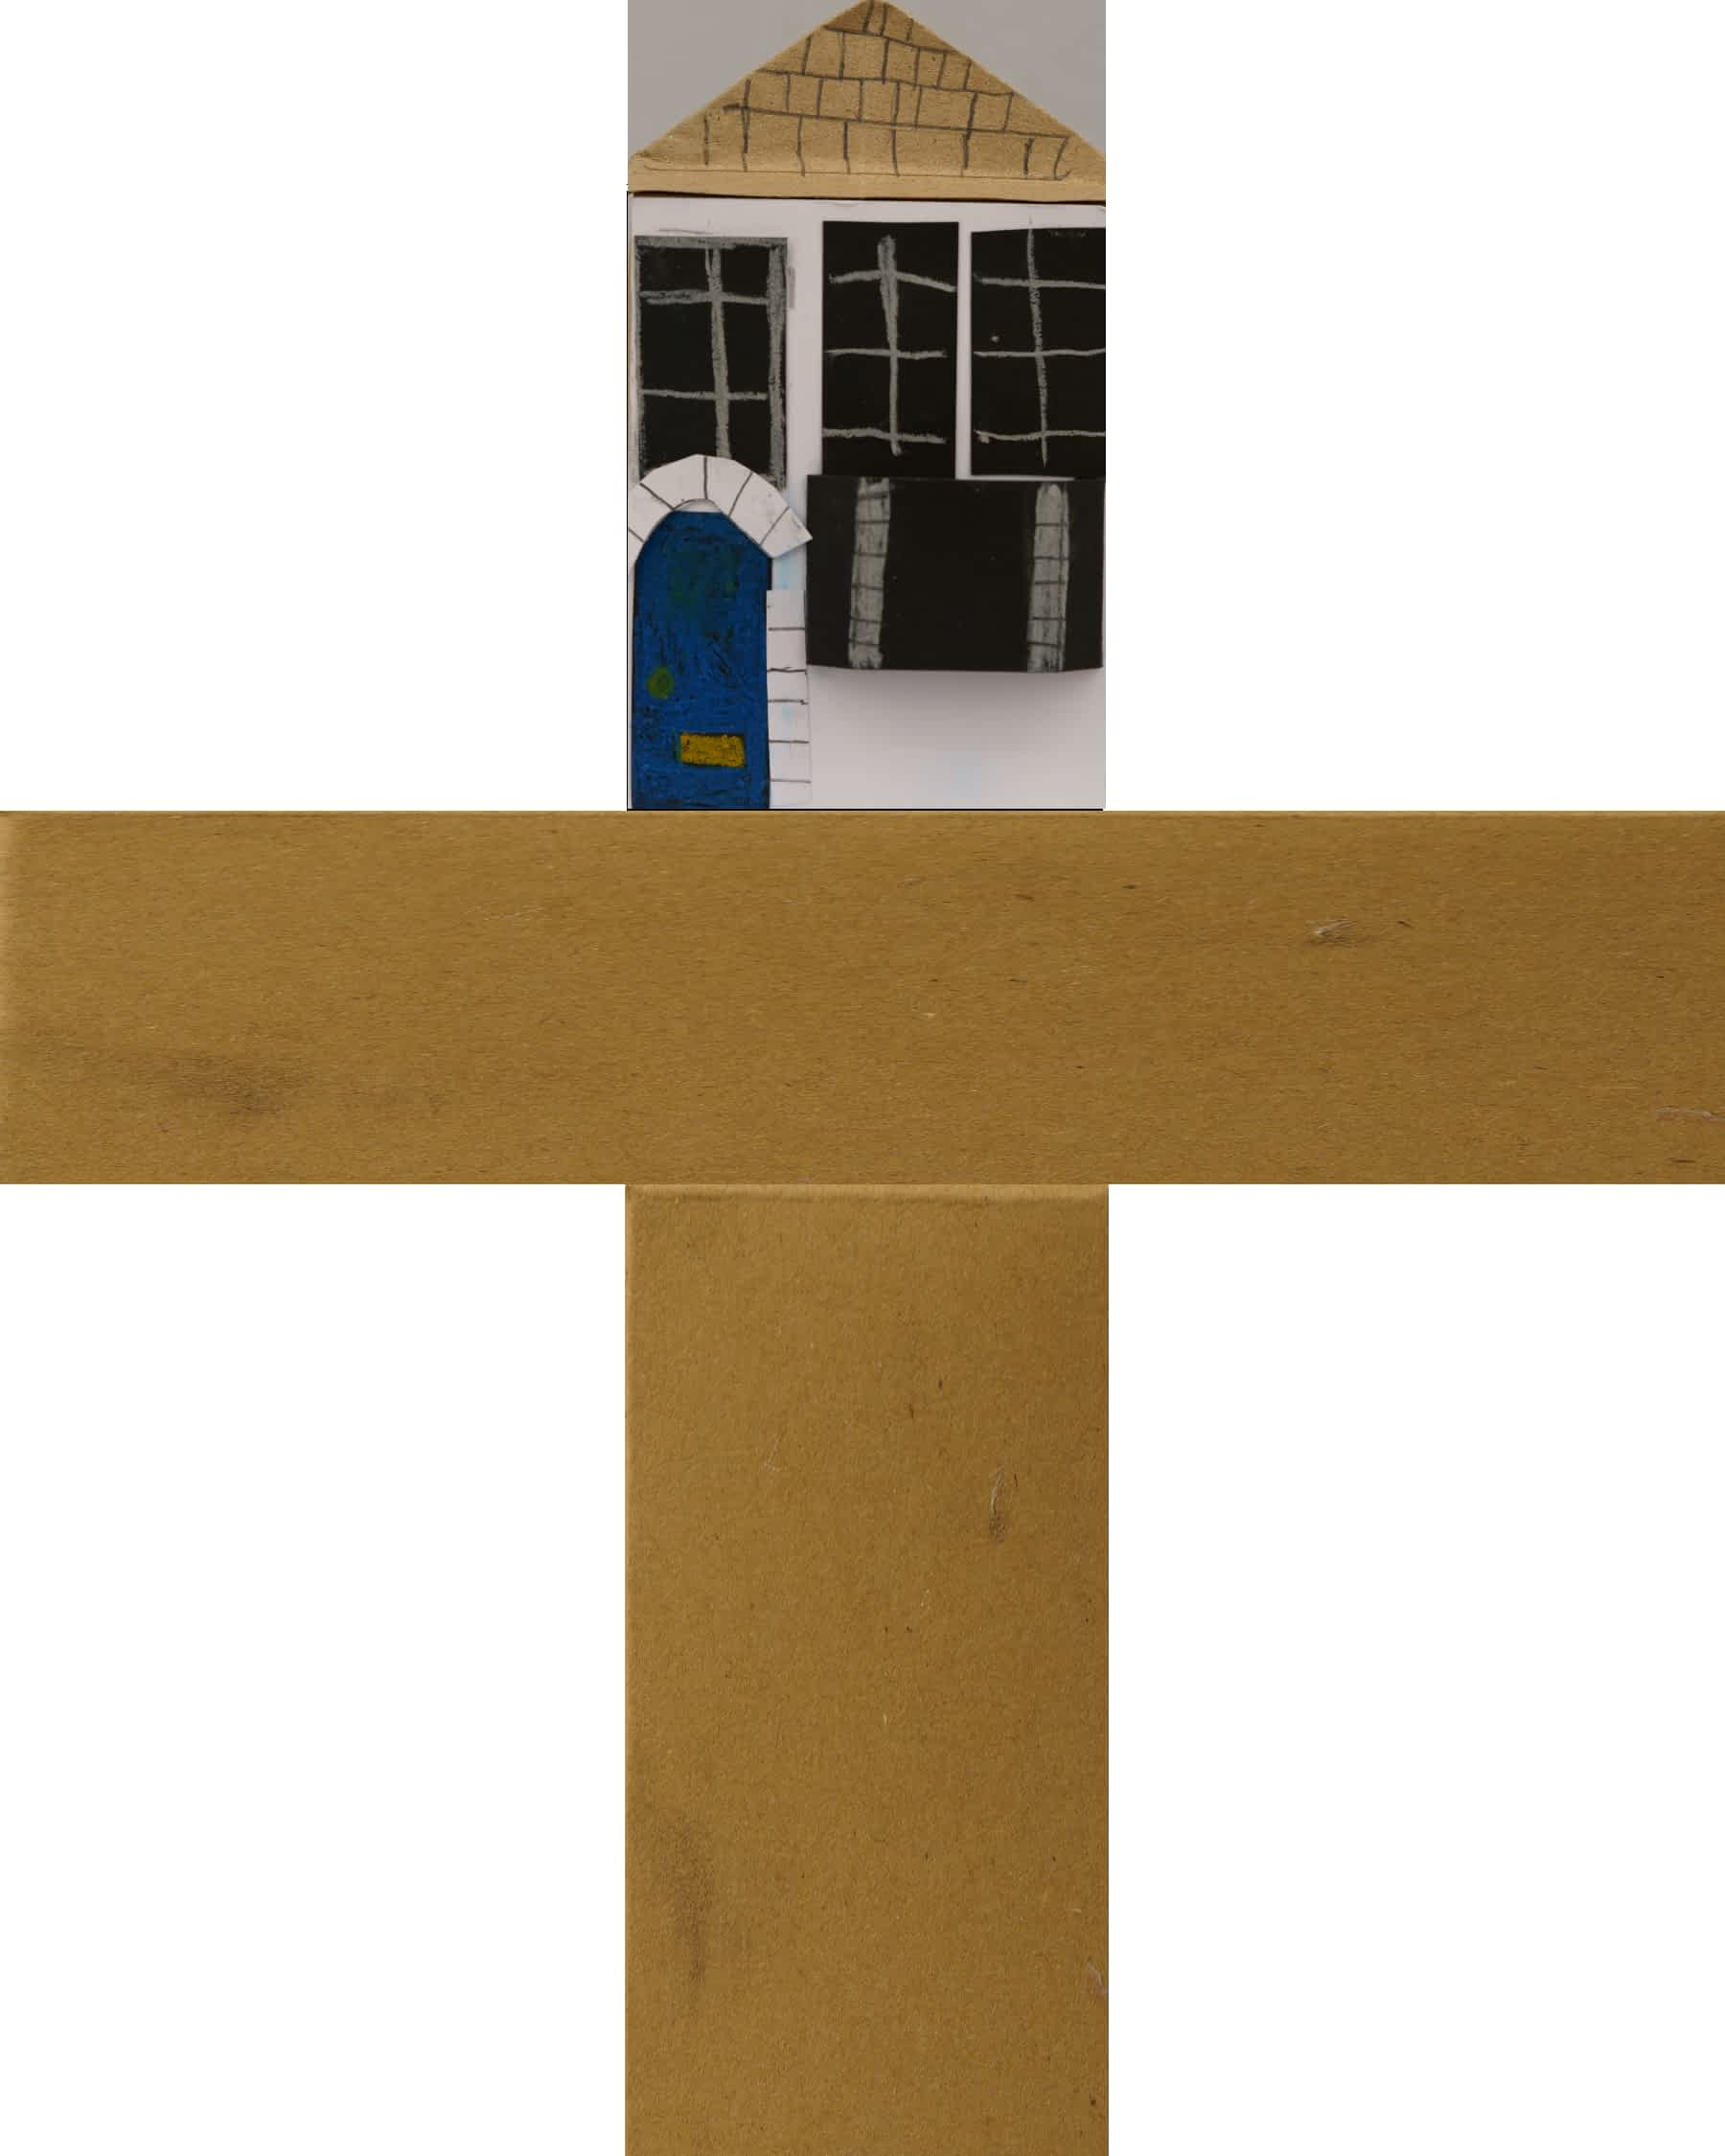
\includegraphics[width=0.49\linewidth]{images/za_tex.jpg}
\caption{Example of unwrapped texture of house} \label{fig:pattern}
\end{figure}


After all the houses had been photographed, the next step was to create the
texture for each 3D model. This was done using the photo editing software
paint.net \cite{paintnet}. First of all, a rough blueprint (see
Figure~\ref{fig:pattern}-left) of each house had to be drawn with
approximately the right measurements so as to avoid distorting the texture
when applying it to the mesh. The images on each side were cropped to fit in
this blueprint as illustrated in Figure~\ref{fig:pattern}. The resulting
textures were then imported into Blender. The 3D models were UV Unwrapped and
aligned with the texture. The final 3D model is shown in
Figure~\ref{fig:3Dhouse}. 




\begin{figure}[ht] \centering
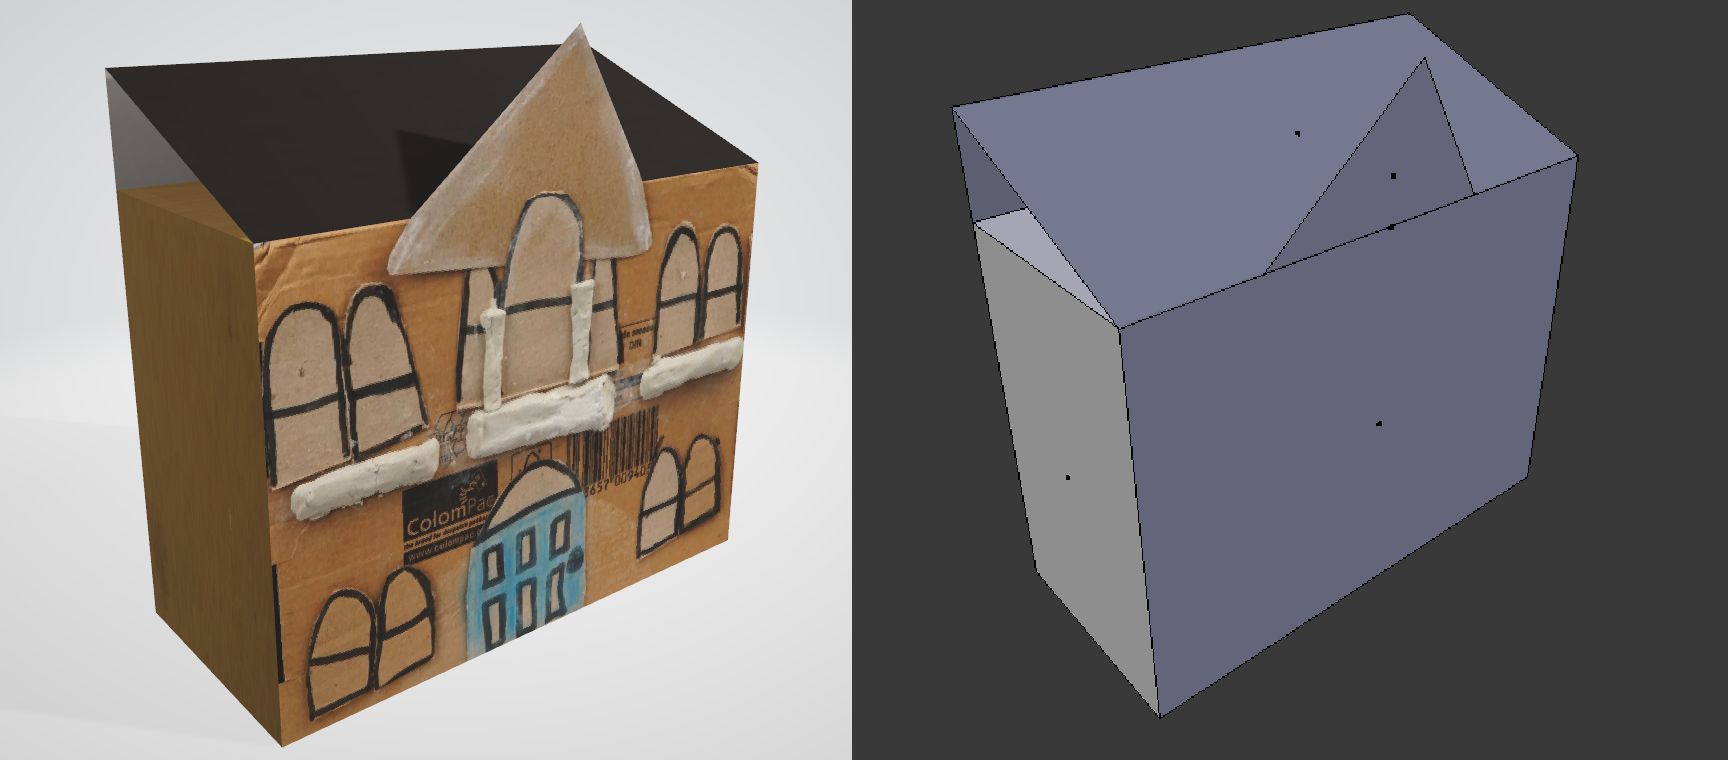
\includegraphics[width=\linewidth]{images/models.PNG} \caption{3D model
of houses with and without texture} \label{fig:3Dhouse} 
\end{figure}

A further modelling task was to produce an animation for each 3D model. This
animation simulates the house `roof' opening and closing in a similar way
which people can open and close the physical box. This was implemented using
keyframes and transformations on the roof sub-objects, and each animation
lasts for 60 frames. Four animations were modelled which correspond to the
four different states a house can be in: 

\begin{itemize} 
  \item \textbf{Open:}
The roof has been rotated 180 degrees by its base, exposing the inside of the
box. 
\item \textbf{Opening:} Transition animation interpolated between open
and closed. 
\item \textbf{Close:} The initial state.  
\item \textbf{Closing:} Transition animation interpolated between closed and open. 

\end{itemize}


The drawings and other written content inside the boxes were scanned using a
flat-bed scanner. Figure \ref{fig:drawingmaps} shows examples of this digital
content. Further editing was done to the images in order to blur personal
information, for example names and addresses. The images were applied as
textures to 3D planes so that they can be visualised as a 3D model.

\begin{figure}[ht] \centering
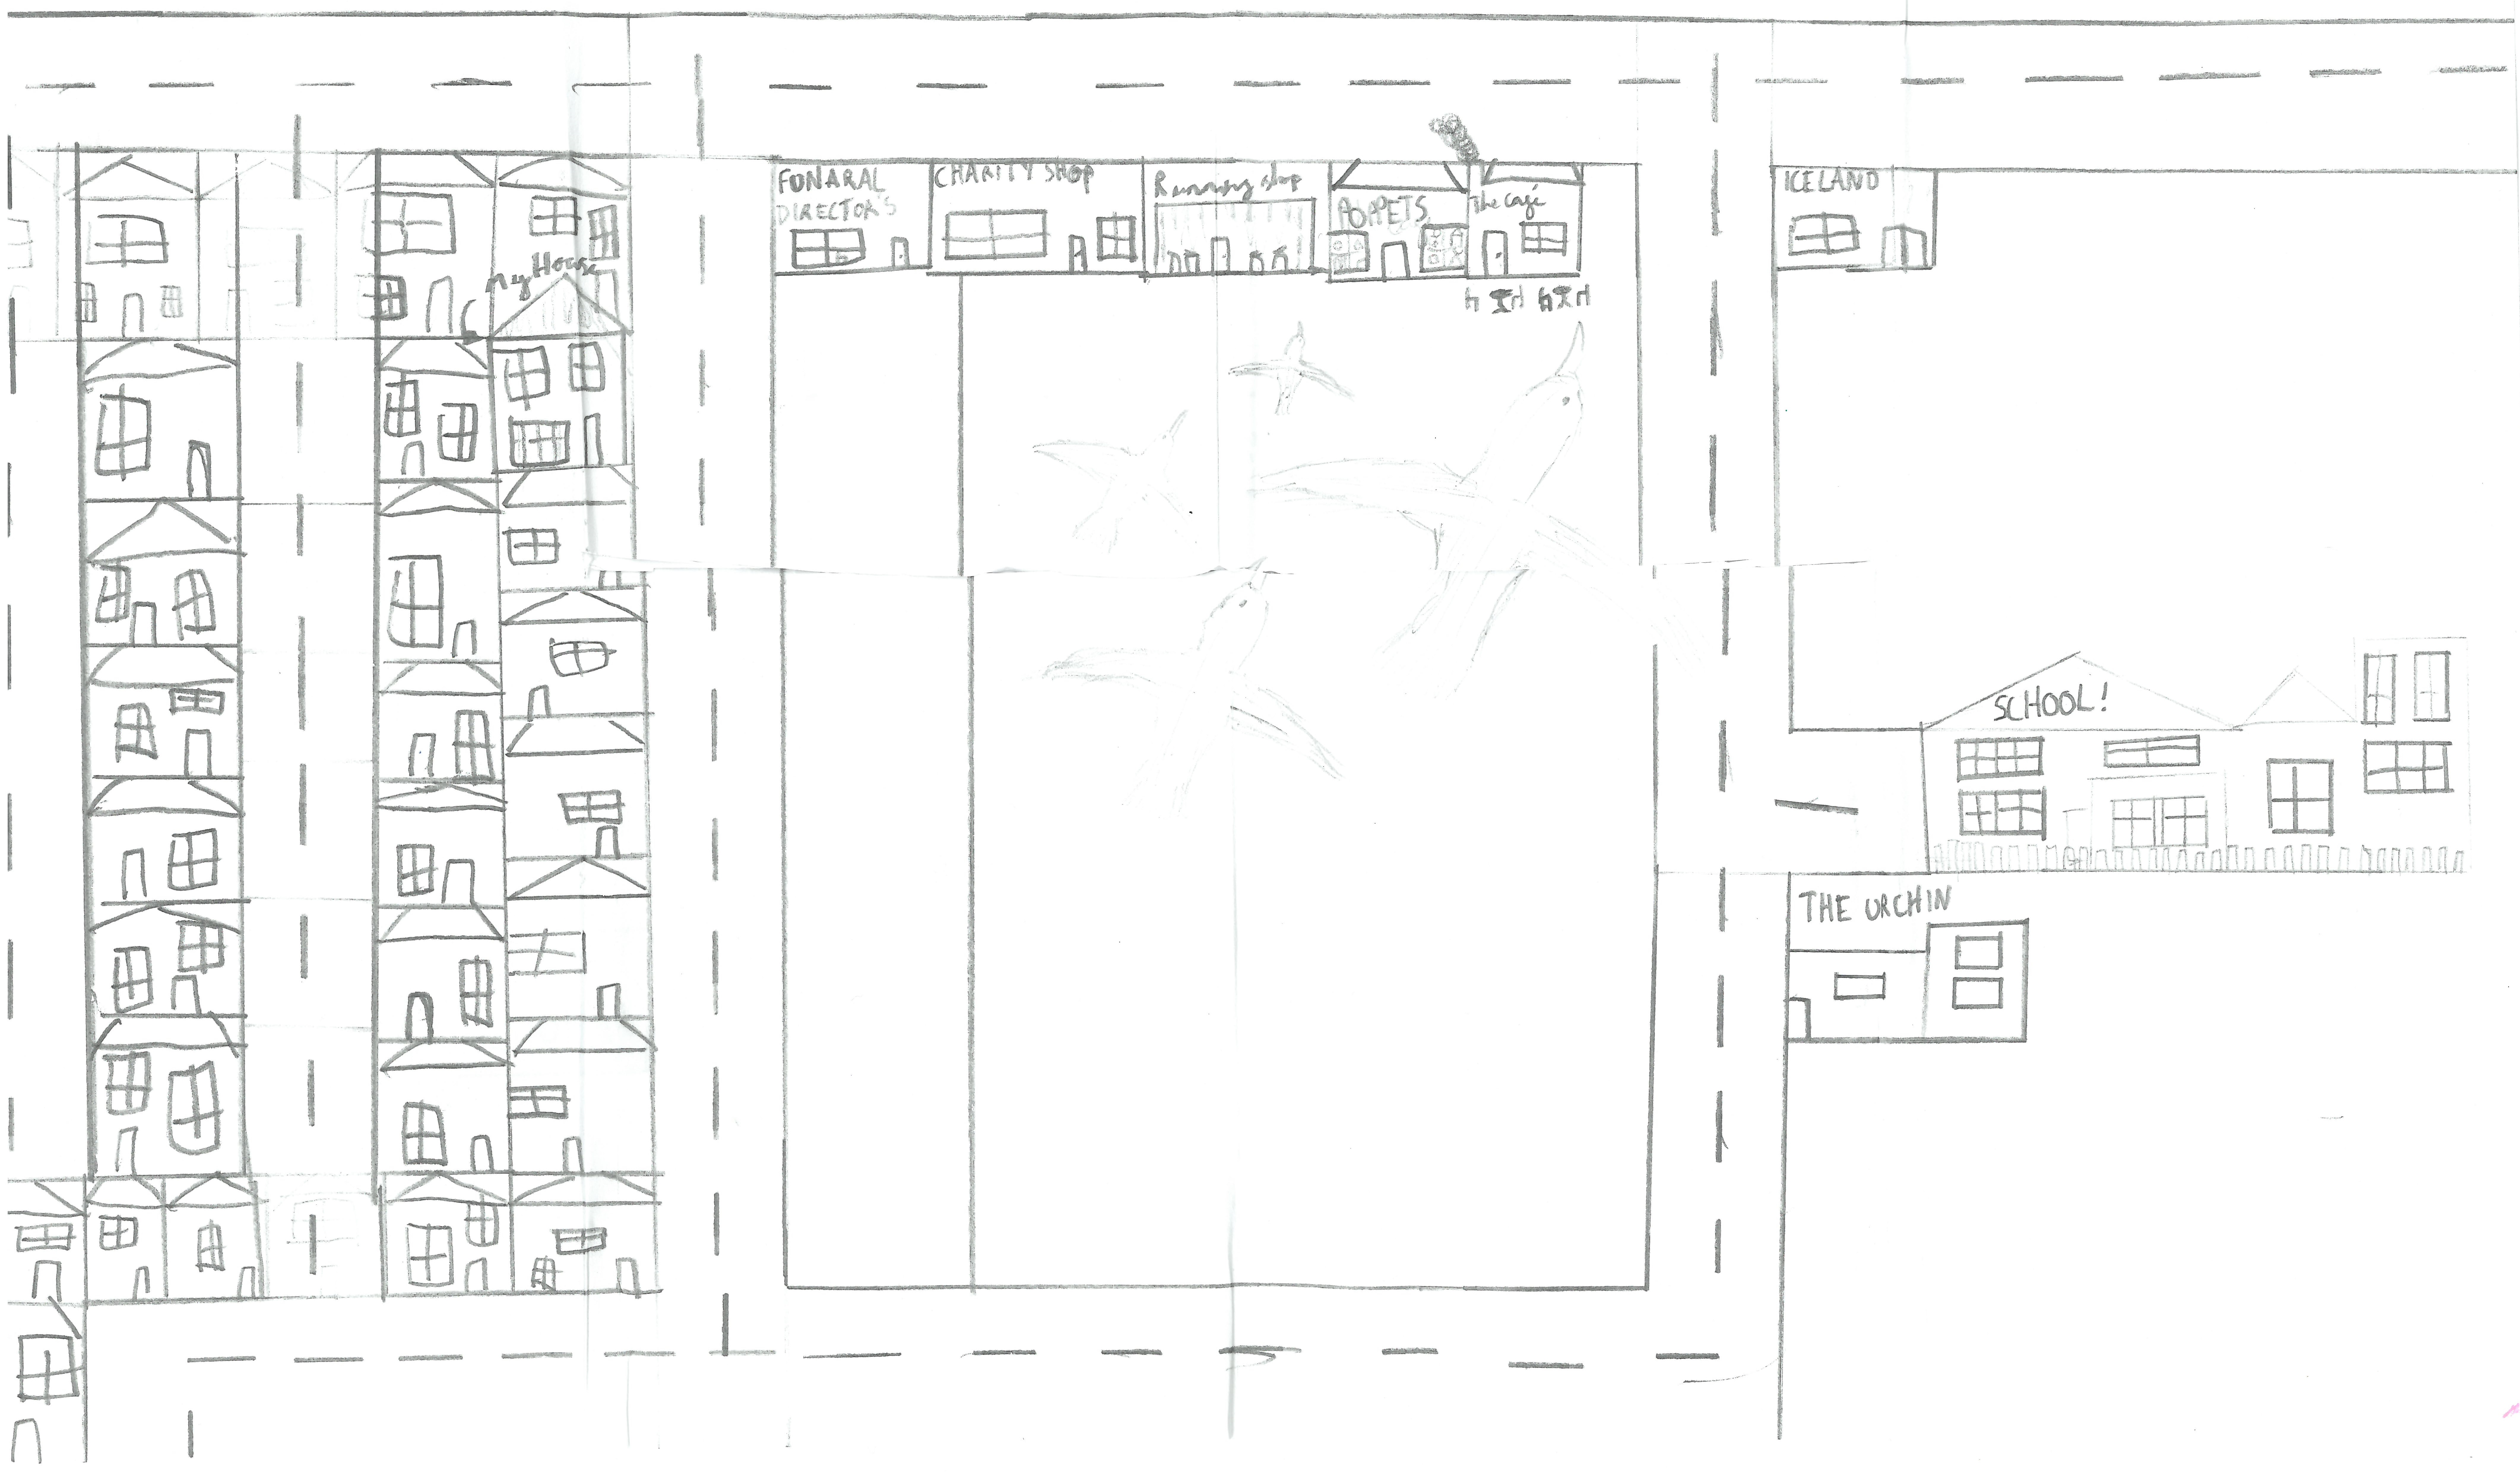
\includegraphics[width=0.6\linewidth]{images/lkp1.jpg}
\includegraphics[width=0.6\linewidth]{images/mgp2.jpg}
\includegraphics[width=0.6\linewidth]{images/fhp1.jpg} 
\caption{Drawings
of children detailing local geographies, journeys from home to school and
objects in the environment.} \label{fig:drawingmaps} 
\end{figure}

Moreover, objects crafted in clay were 3D scanned using the Artec3D handheld
3D scanner. Additional 3D models were accessed from a relevant project
\cite{14f05b94a1844f5e850c87fc9d042c59}. This project undertook the
digitisation of public sculptures in the same geographical area using a
crowdsourcing approach and published the resulting 3D content on the web.

All content had to be post-processed in order to make it web-ready for the AR
experience. This required developing workflows for the production of 3D meshes
to be of suitable size/quality for distributing them over the web. 

Moreover, the textures had to be optimised for web delivery as the initial images were
produced with very high resolution and file size. This was done by running
them through the imageoptim web service \cite{ImageOptim}.  
%Furthermore, all images had to be resized to dimensions which were powers of two (e.g.
% 2048x2048, 512x1024) to facilitate loading.  The images produced used a final
% resolution of 96dpi.

The glTF file format was used for encoding the 3D models and their animation
for the AR experience. glTF (GL Transmission Format) is a common specification
for the efficient transmission and loading of 3D scenes and models, especially
by web applications \cite{khronos}. It reduces both the size of 3D resources
and the execution processing required to decompress and use them. It stores a
full scene description in JSON format, which includes node hierarchy, cameras,
and materials and it also contains descriptor information about animations and
meshes.

% The following section will describe the implementation details of the AR
% application.

\subsection{Web based Augmented Reality (AR)} % %talk about how it was put all

In order to make the AR maps easily
accessible, the research makes use of an \emph{Immersive Web} approach, which
refers to virtual world experiences hosted through the browser, covering both
Virtual Reality and Augmented Reality experiences developed for AR-enabled
devices \cite{imweb}. The WebXR API is currently the experimental
specification for both augmented reality and virtual reality devices
\cite{webxr}.

Currently, web-based AR technologies make use of API such as WebRTC and WebVR
to enable to deliver AR through the web browser. Other frameworks which are
available include Argon.js \cite{Argon.js}, AR.js based on A-Frame
\cite{aframe}, Awe.js, \cite{Awe.js}, 8th Wall \cite{8th}. All of these
frameworks make use of Javascript and some of them offer markerless
capabilities (e.g. 8th Wall) through a paid service.

Although AR installed as an application on a mobile device often offers better
performance, it was deemed that a web-based approach will enable more people
to access the experience from a diverse set of devices and platforms. For
instance, frameworks such as Vuforia \cite{Vuforia} are not web based and
require of payment to be used without watermarks. 
% %However, they are
% markerless and offer high stability and many extra features. Nevertheless,
% they require to be installed as an app and the heritage sector is increasingly
% reluctant to use this approach.

Ar.js and A-Frame were used as a framework to develop the web-based experience
as they are open source solutions. A-Frame is an open-source web framework for
building both Virtual Reality (VR) and Augmented Reality (AR) experiences
based on Three.js. A-Frame is an entity component system framework and it
allows to create 3D scenes using HTML and Javascript. Most 3D operations are
performed by A-Frame in memory with minimal overhead and are rendered with
WebGL \cite{webgl}, which binds to OpenGL or Direct3D. A-Frame is meant to
give suitable latency and framerate with browsers, such as Firefox with WebVR.


\begin{figure}[ht] \centering
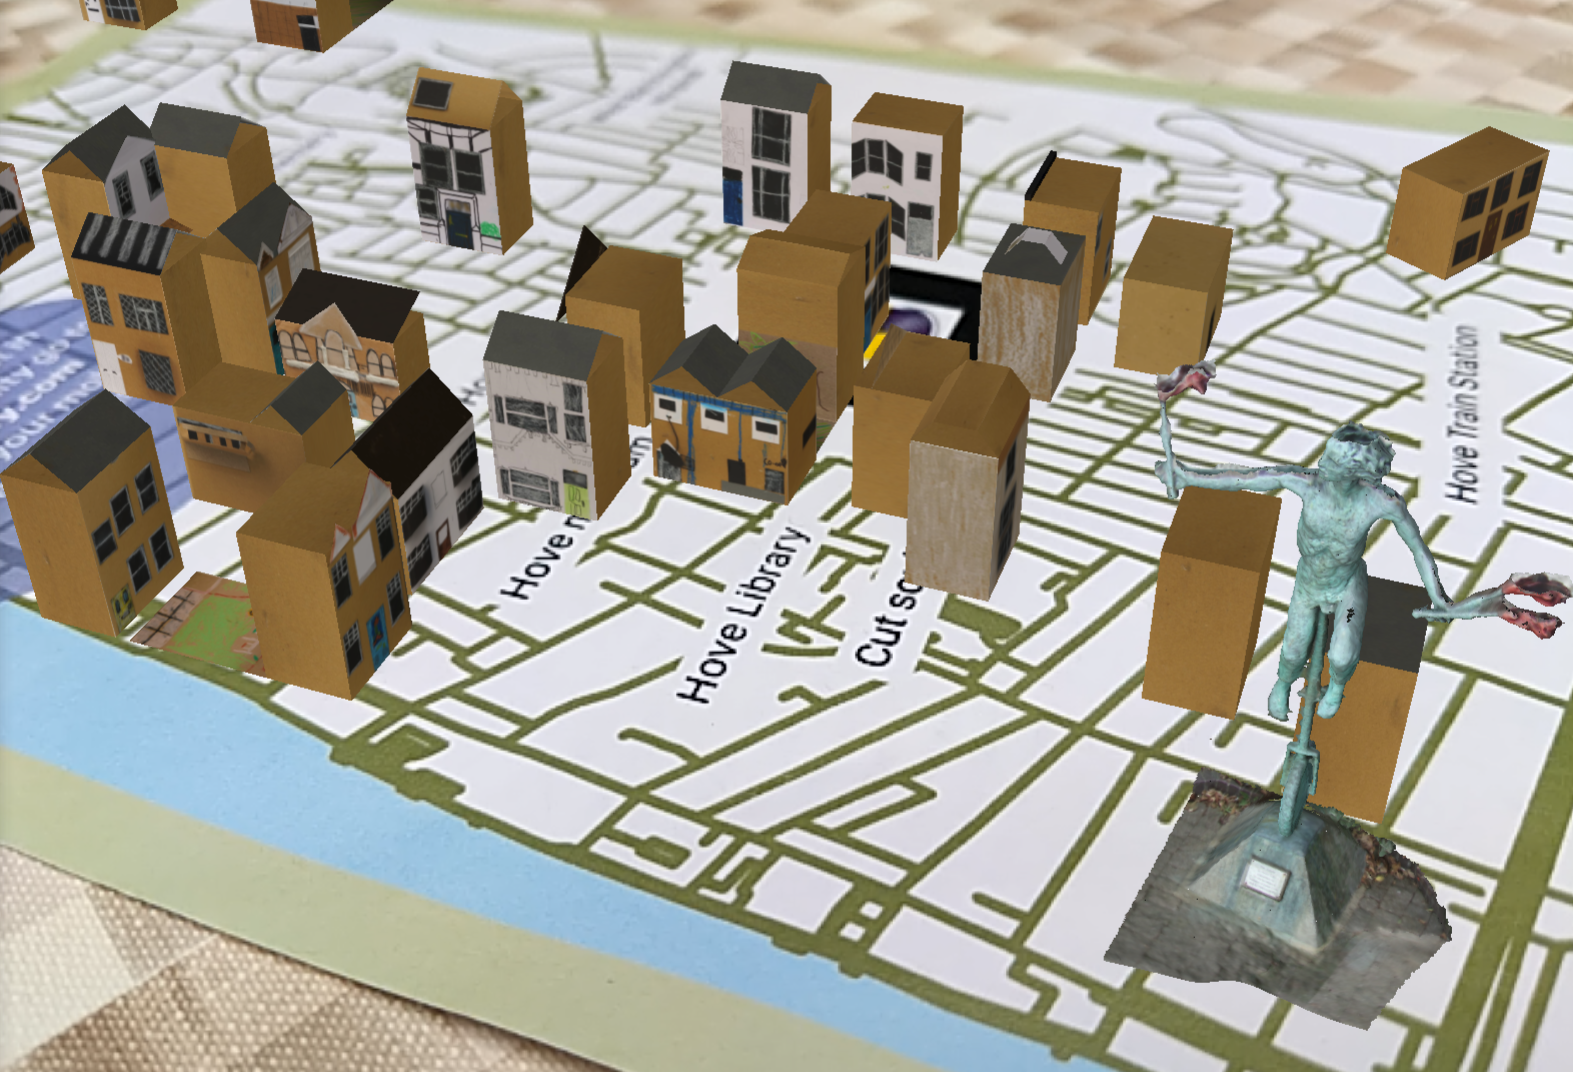
\includegraphics[width=0.6\linewidth]{images/ARcontentw_sculpture.png}
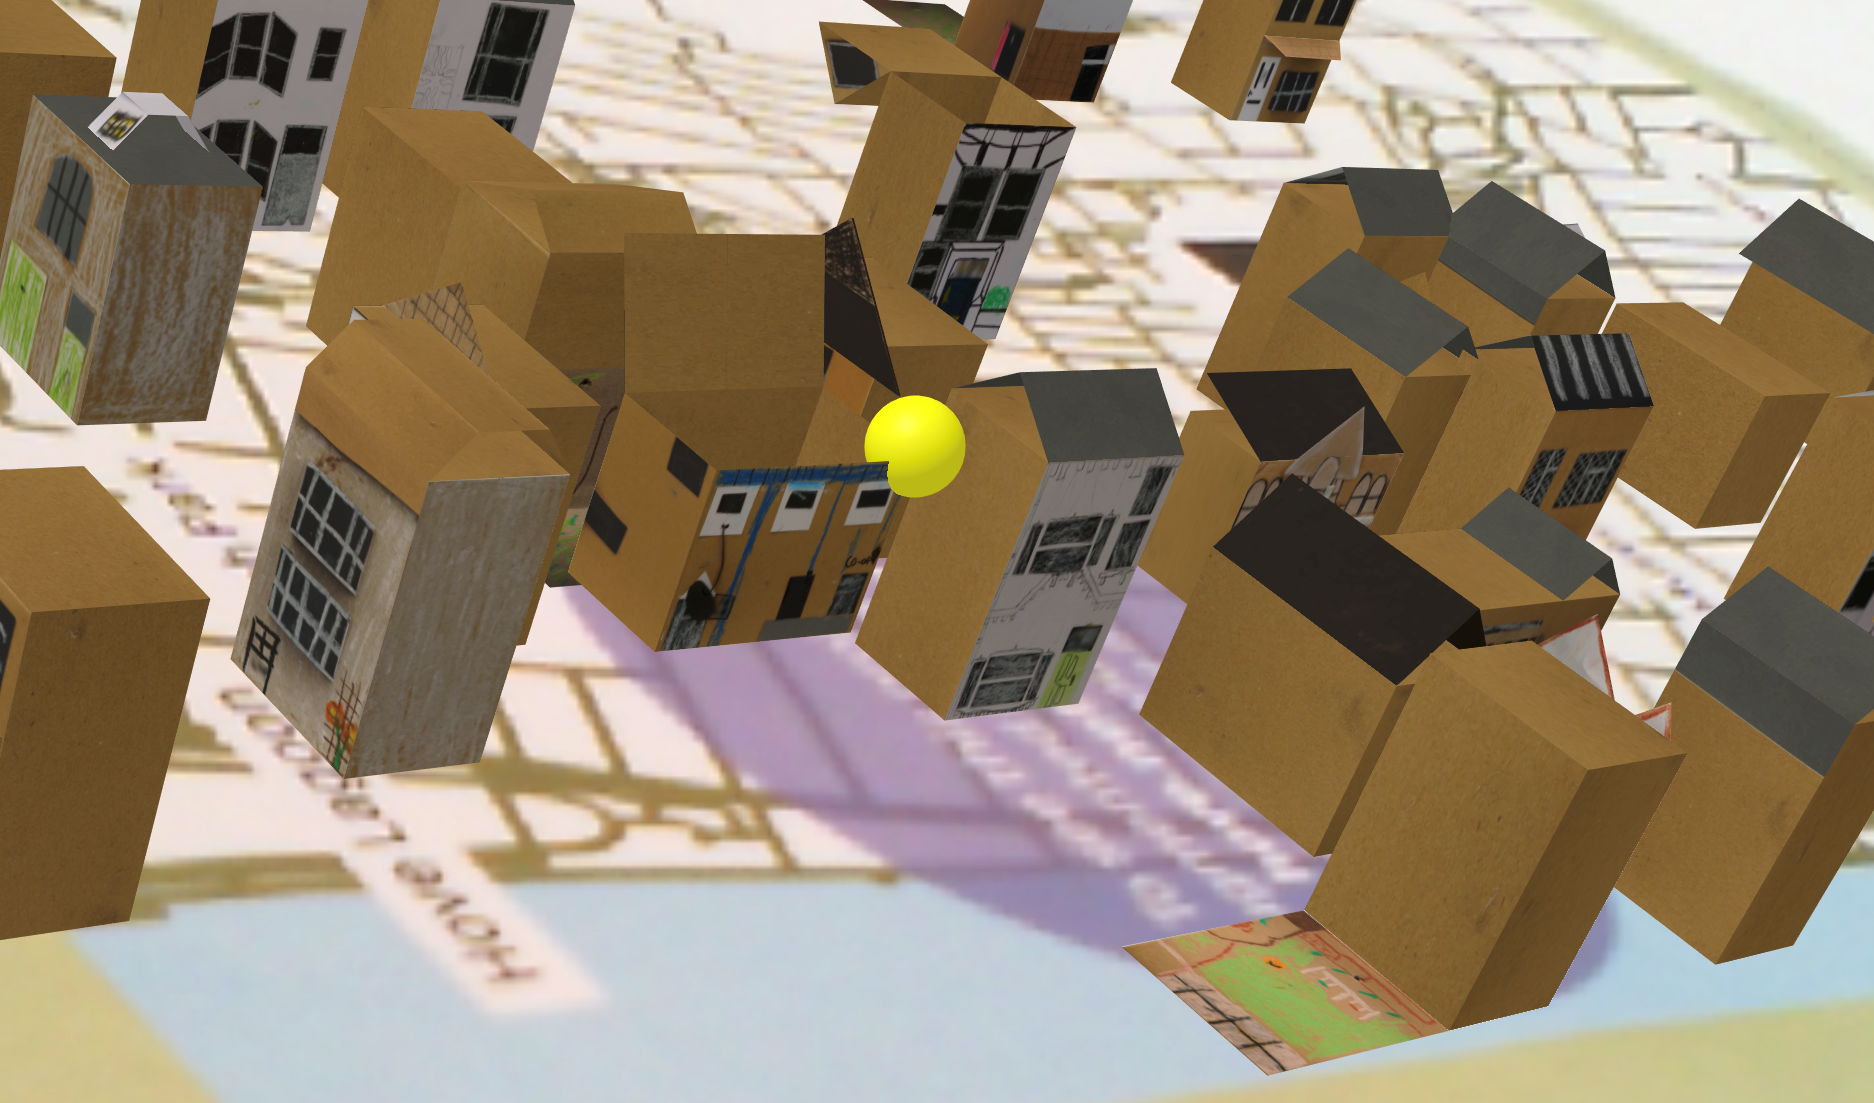
\includegraphics[width=0.6\linewidth]{images/animationARexperience_zoom.png}
\caption{AR Map experience showing the different house models and a sculpture in the geographical area (left),
 animation to open the house is triggered when the user taps on a house model providing a visualisation
 of the child's map shown in Figure~\ref{fig:drawingmaps}  } \label{fig:ARexperience}
\end{figure}
 
In the project the Aframe raycaster is used, which is built
on the Three.js raycaster. On collision with an object, the raycaster triggers
an event on said object. 

The AR.js API is used to render all elements of the scene which includes the
houses and other additional 3D content. The marker on the printed map is used
to position the 3D scene on the printed map (see
Figure~\ref{fig:ARexperience}-top). In order to enable user interaction with
the 3D models, the Three.js raycaster is used. The system triggers a different
behaviour according to the type of object that is clicked: 

\begin{itemize}
\item When the user taps on a house, the animation to open or close the house
is triggered (see Figure~\ref{fig:ARexperience}-bottom). After playing the
animation, the content which belong to each box is displayed on the Universal
Viewer \cite{uv}. The implementation includes the capability to add hyperlinks
to direct the user to explore further information on the web. 
\item When the
user taps on a 3D model of a sculpture, the object acts as a hyperlink to
relevant information, which has been curated by a researcher.  
\end{itemize}

% At this point, the desire to give more details on the children's maps gave
% us the idea of adding an information button that would allow us to access
% this supplement. The first step was to add a url to the index.html file for
% homes that needed more information.  Then, in the viewer.html file, a button
% was added after the close button (which allows you to return to the home
% page).  The next step was to add an event listener to this button to give it
% a function. This function was to open a new window with a url. And finally,
% when the house did not require any further information, the button should
% not be visible to the user. What has been managed by defining a classList
% equal to "hide" at the button

The framerates and latency achieved with the current development were tested
in various platforms (see Table \ref{table:framerates}). Latency is an
expression of how much time it takes for a packet of data to get from one
designated point to another. As expected, the framerates vary with the
processing power and graphics card capabilities. The highest framerate
achieved is of 60 frames per second (fps) on a mobile phone (see row 2 in
Table~\ref{table:framerates}). Although the responsiveness on mobile phone for
racytracing performed worse on a mobile device than on a laptop or PC.

High framerate and low latency is the ideal and these seem to have a direct
correlation to the CPU/GPU for mobile devices. 60fps/16ping seems to be the
best across all devices. However, the fact that a Google Pixel 2 and 3 both
have the same despite differences in CPU/GPU suggest improvements are minor
for these newer models. The lower framerate shown by the MacBookPro
and ASUS Zenbook indicate that the APIs are well optimised for mobile
architectures.

%One possible reason for this could be due to the framerate of the camera
%(newer phones have a high quality, high framerate camera which is better than
%laptop webcams or tablets).

% \begin{table}[h] \centering 
% \begin{tabular}{|p{90px}|c|c|} \hline Device & 
% Framerate (fps) & Latency (ping)\\  \hline \hline 
% Google Pixel 3 (Octa-Core,
% Adreno 630 1 MB, 4 GB LPDDR4X) &  60 & 16\\ \hline
%  Google Pixel 2 (Octa-core,
% Adreno 540 1 MB, 4 GB LPDDR4X)  &  60 & 16\\ \hline
% Pocophone F1 (Octa-Core, Adreno 630, 6 GB) & 60 & 16 \\ \hline 
% MacBook Pro
% (Intel Core i9, Radeon Pro Vega 20 4 GB, 32 GB DDR4, 720p camera - 30 fps)  &
% 50 & 17\\ \hline 
% Nexus 5X (Hexa-Core, Adreno 418 512 KB, 2 GB LPDDR3) & 32 &
% 42 \\ \hline  
% Nexus 5X (Hexa-Core, Adreno 418 512 KB, 2 GB LPDDR3) & 32 & 42
% \\ \hline 
% ASUS ZenBook UX330UA (Intel(R) Core(TM) i5-7200U CPU, RAM 8 Go) & 30
% & 20\\ \hline 
% Galaxy Tab S3 (Quad-core, Adreno 530, 4GB of RAM) & 18 & 50\\
% \hline \end{tabular} 
% \caption{Testing web-based AR application in various
% devices of scene containing 1,176 triangles} \label{table:framerates} 
% \end{table}


% \subsection{Link to additional information on objects}


%-------------------------------------------------------------------------
\section{Preliminary evaluation} \label{eval} An evaluation took place before
the start of the project to provide a baseline from which to measure the
project outcomes. During this survey, children were asked about their
well-being, confidence and overall resilience in life. Another evaluation took
place after the school workshops, which showed that the proposed process can
lead to children reporting feeling better about themselves and their mood. For
instance, there was a 45\% increase in children reporting feeling very happy,
18\% increase in children reporting liking themselves, a 15\% increase in
children reporting that they coped with difficult situations happily or very
happily, and a 15\% increase in children feeling liked by other people. During
this evaluation, the AR Maps were not evaluated as these were not yet
developed.

In July 2019, a 'celebration' of the artwork and the children's journey took
place at the Hove museum (UK). During this day, all children were invited to
bring their families and friends to show the artwork and talk to the
researchers developing the AR application. The setup in the museum included
three areas: 1) an area to display the artwork and to engage with the AR
experience (see Figure \ref{fig:museum}-top), 2) an area for visitors to
engage in the creative process for creating their own journeys (see Figure
\ref{fig:museum}-bottom), and 3) an area for visitors to experience a creative
application in Virtual Reality. It was considered that this provided a good mixture
of hands-on and creative digital activities to engage visitors.

It was the first time the families and friends had seen the artwork and the
first time the children had seen the AR Map experience. Hence, we printed a
large amount in 80 gsm recycled paper and we distributed them amongst the
visitors of the museum and sent extra copies to the school.

\begin{figure}[ht] \centering
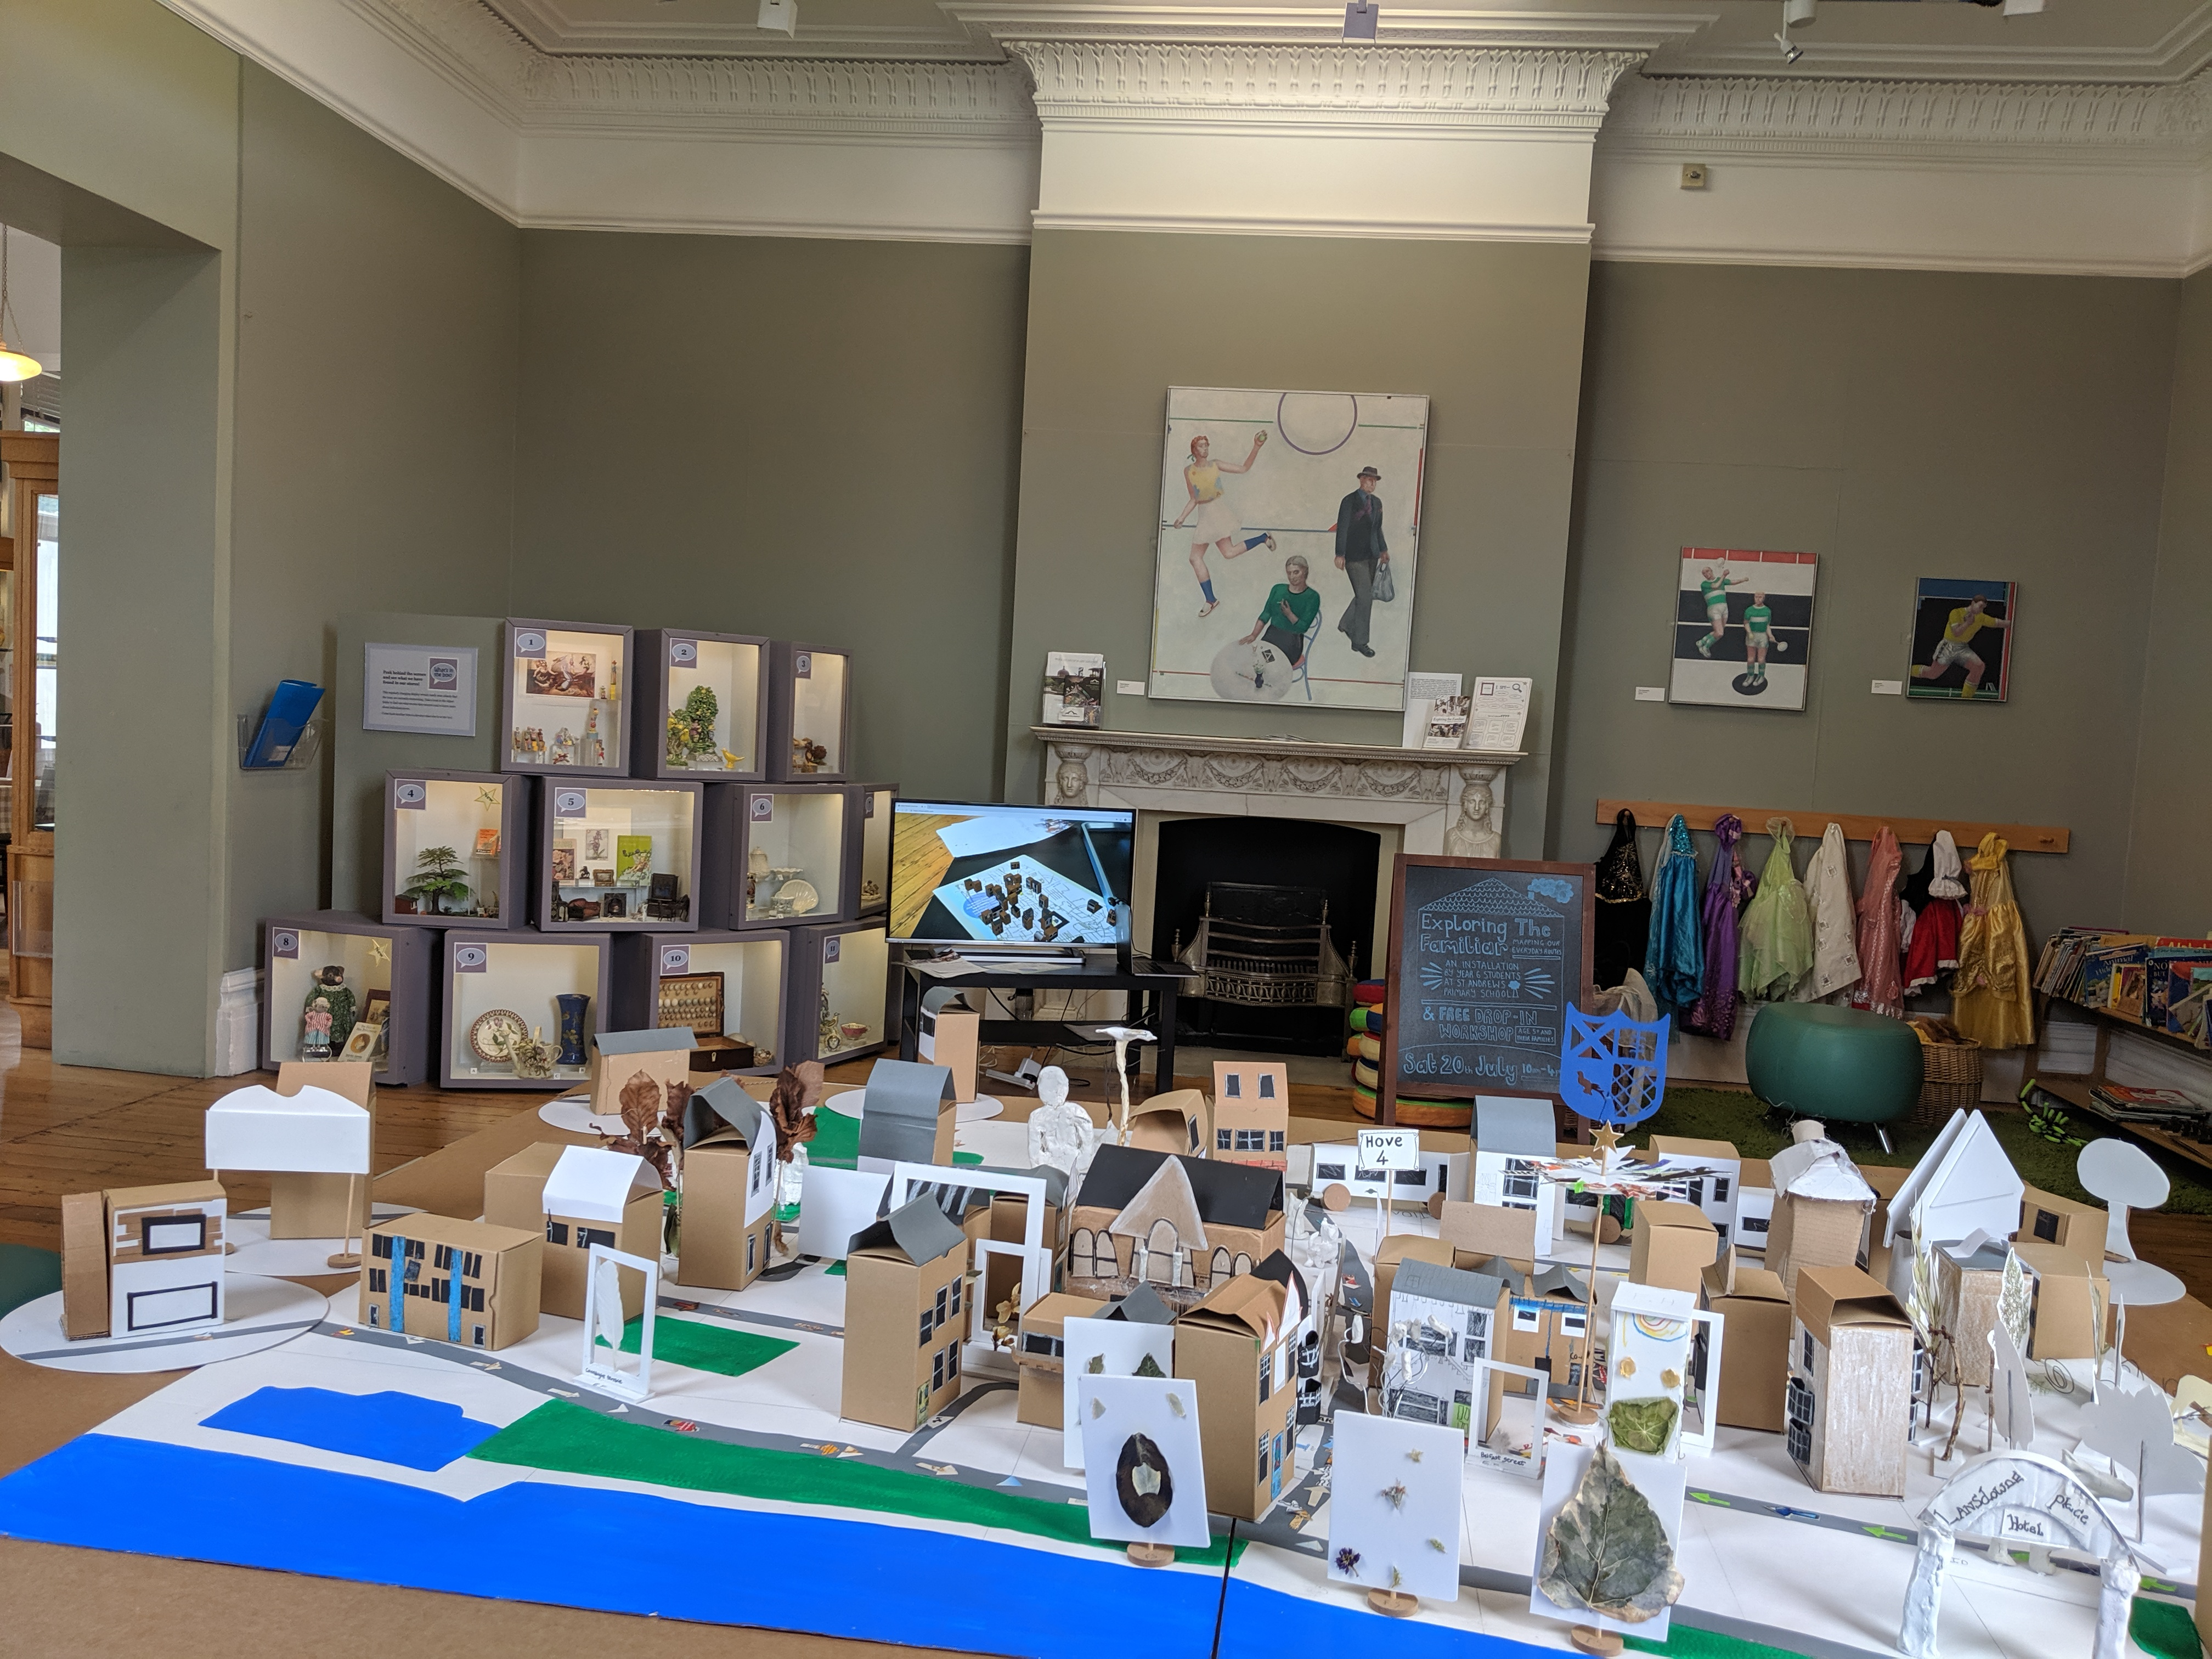
\includegraphics[width=0.6\linewidth]{images/IMG_20190720_103105.jpg}
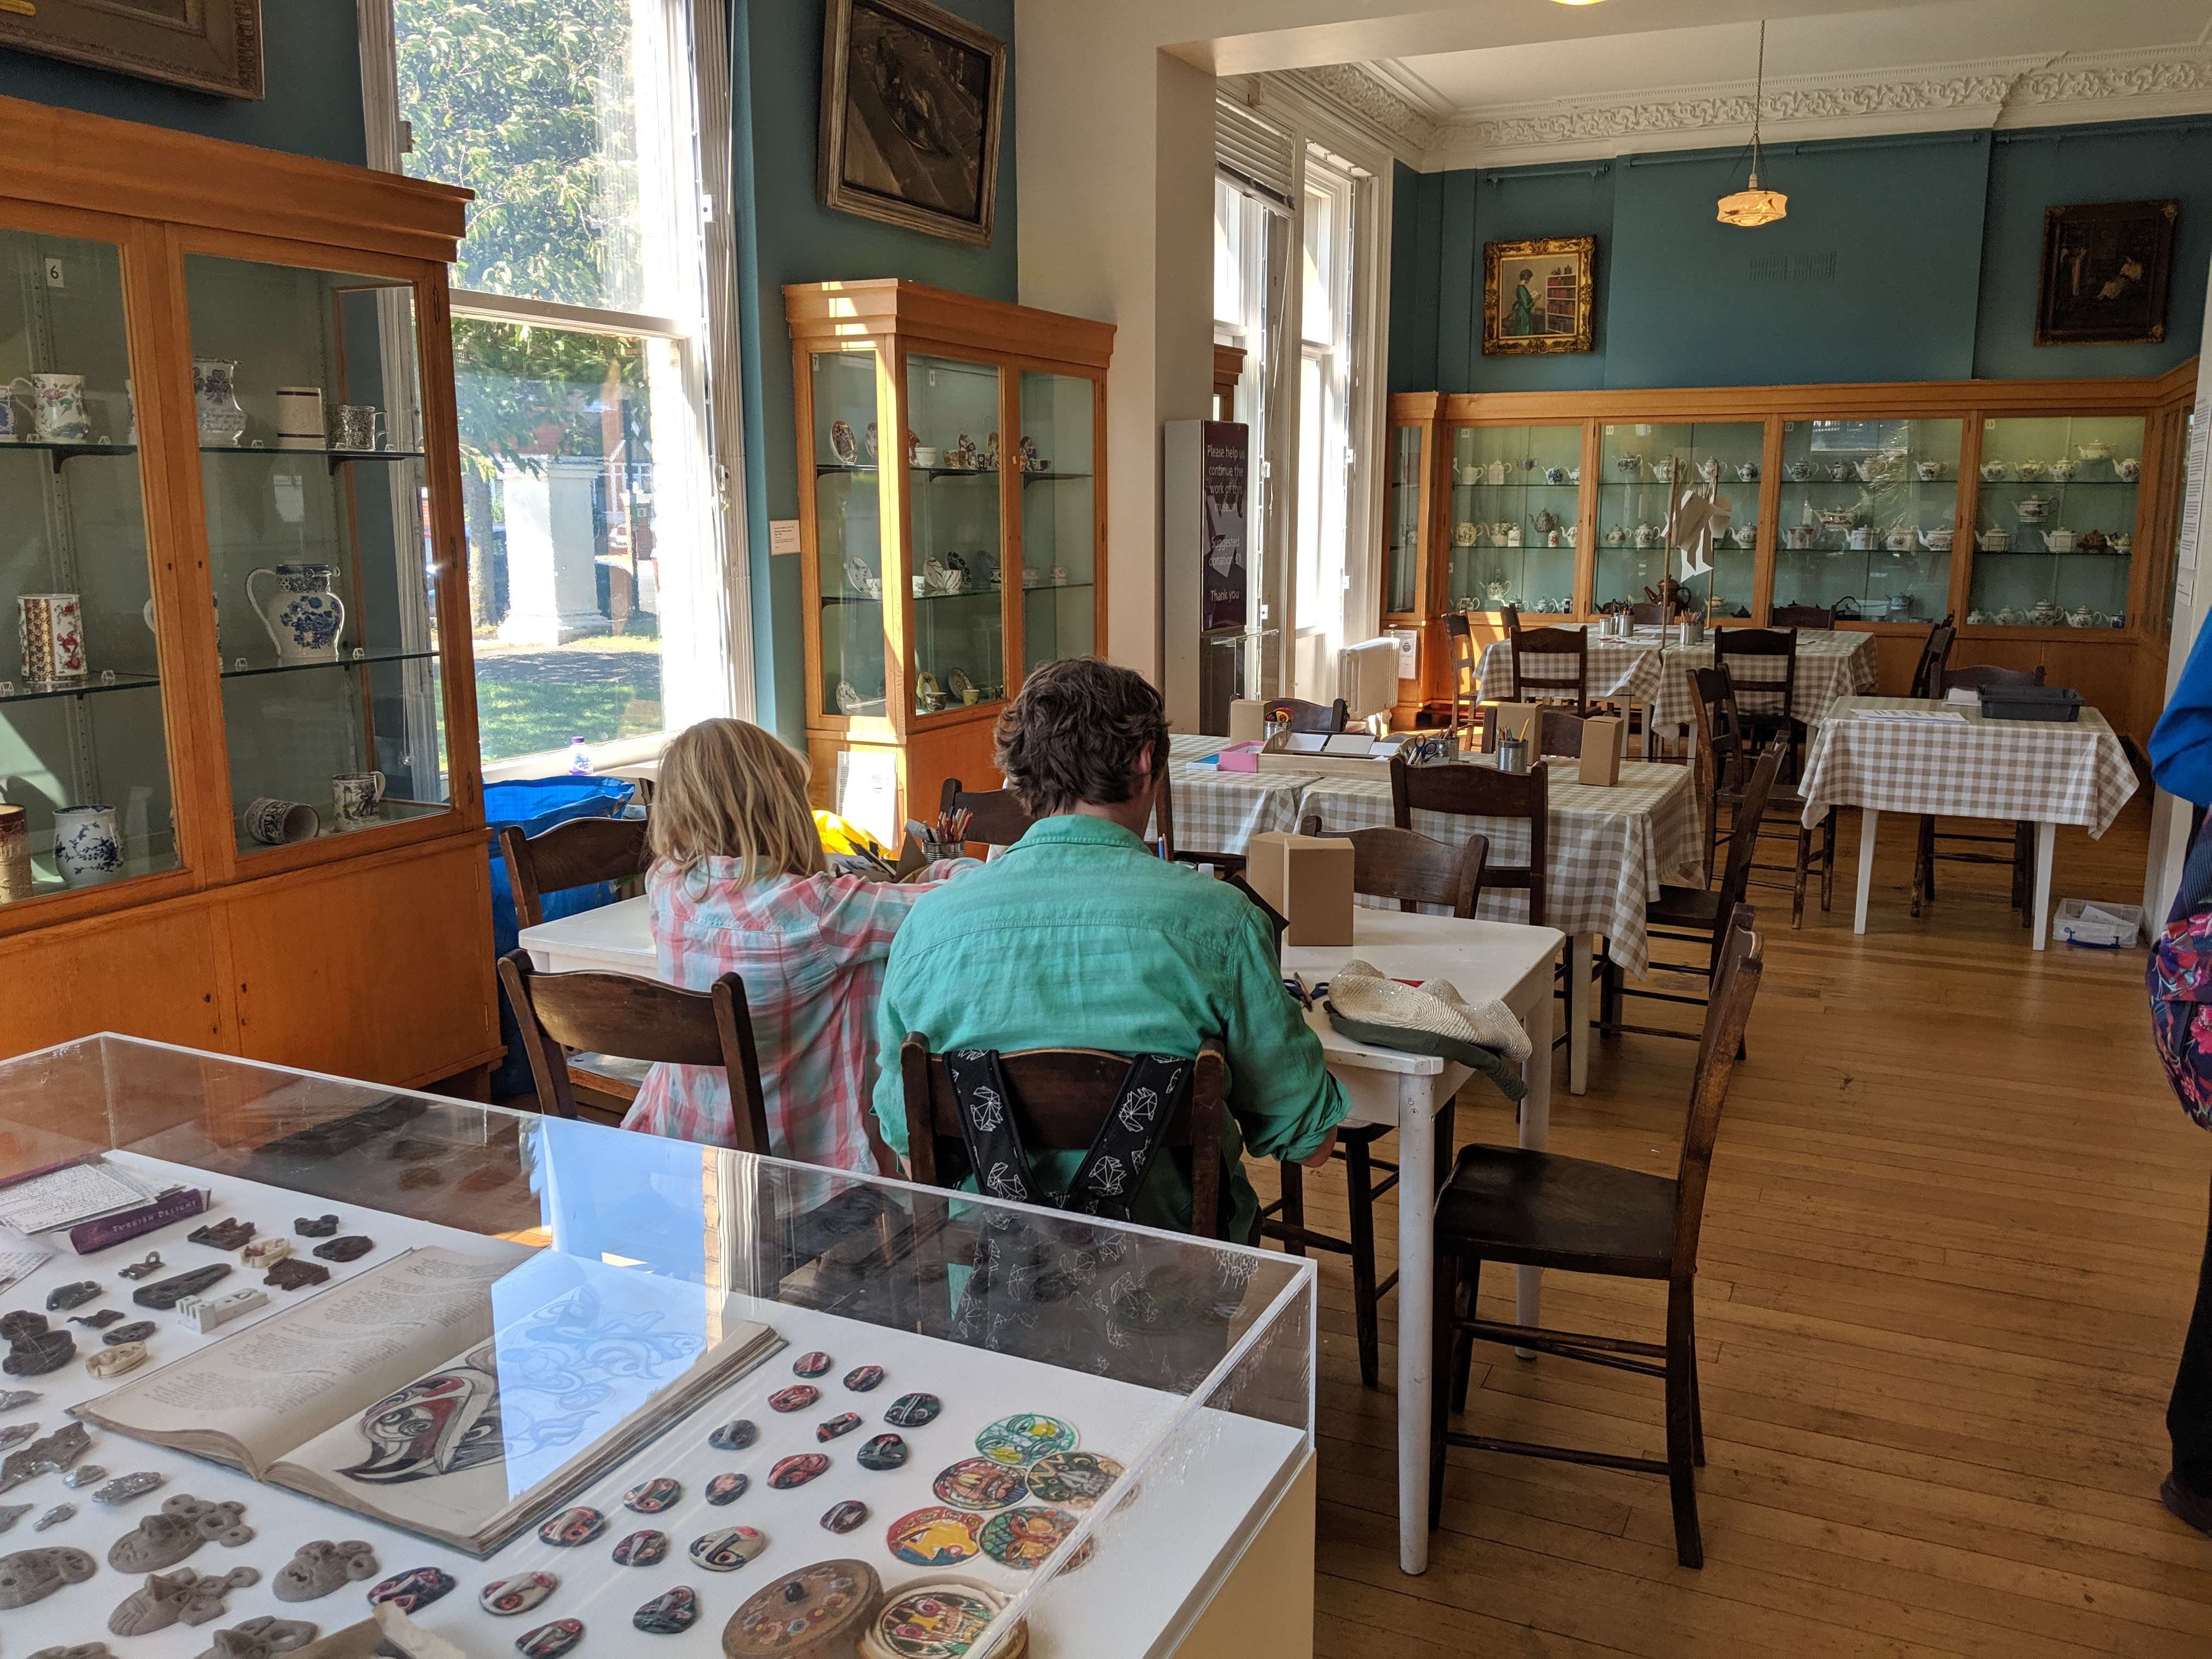
\includegraphics[width=0.6\linewidth]{images/IMG_20190720_151644.jpg}
\caption{Setup at the Hove museum for the celebration of the artwork and
release of the AR application, top) area with the original map, bottom) area
where people can engage in the creative process} \label{fig:museum}
\end{figure}
 
Initial feedback from the children provided evidence that the experience was
engaging because of the Augmented Reality aspect. Children were keen to test
the printed map on their phones and look for their house and their stories.
Most children were very proud to see the content they had produced being
rendered on the screen when they touched on the house and were happy to tell
others about the journeys that they made every day. For others who had no
direct connection to the children, the AR experience was very interesting.
They would randomly tap on houses and inspect the content others had created.
 
 During the testing, we also found technical issues with the AR aspect. The
 most common issues were related to size of the screen to experience a large
 amount of visual content and the responsiveness of smart devices with less
 powerful CPU/GPU. Despite the cross-compatibility of the AR framework, there
 were also issues with iOS devices including iPhones and iPads. Furthermore,
 the testing also made evident that clearer instructions on the printed map
 were needed. Some people will immediately switch their cameras on (without
 going first to the website) and be surprised that there was no content
 displayed.  All of this feedback is currently being incorporated into a
 second release of the AR Map experience. 


%-------------------------------------------------------------------------
\section{Conclusions} \label{conc} This paper presented novel research for the
development of approaches and technologies which enable communities to
meaningfully engage with their cultural environment in creative ways. Thus,
the paper describes the methodology for deploying the approach which is tested
with a local community in Brighton and Hove (UK). As a result, children
engaged in a creative process to look at their community in new ways and
produce narratives.

The paper demonstrates how mobile and augmented reality technologies provide a
novel element for re-telling these narratives to wider audiences. These
experiences combine physical maps, such as those widely used for tourists,
with augmented 3D using Immersive Web technology. 

Feedback from users demonstrate the potential of these approaches to raise
awareness of the cultural elements of the local area as well as to improve the
well-being and happiness of children who engage in the process. In addition,
the AR elements triggered the curiosity of users to explore the different
narratives, while becoming aware about other people's viewpoints of their local
environment.

Further work involves the usability evaluation of the Augmented Reality aspect
in order to understand how to overcome issues such as latency and
user-friendly access to the content when this is viewed from a mobile device.
Another area to explore is how to ease the digitisation of the material
created, including those objects created in different materials. Children should
become involved in this process as it will enable them to enhance their digital
skills as well as to find novel ways to create links between the material created and
content on the web which is curated by heritage experts. 

%type of experiences can allow community members to experience narratives
%relating to people, objects, sites and events which are of importance to the
%communities that live amongst them.


Ultimately, the research contributes towards enabling communities to
participate in the identification and preservation of cultural heritage. This will 
 facilitate the democratisation and promotion of a better understanding
of the multiple meanings of heritage.


\section{Acknowledgements} We would like to thank Bec Britain and Jo Coles
from Our Future City who co-designed, developed and delivered the workshops as
well as Peter Chivers for supporting the activity. We also thank Karin Janzon,
from Hove Civic Society, for her continuous support in engaging communities in
Hove as well as Kate Howland, who contribute to ideas for the community engagement. 
Finally, we would like to acknowledge the teachers and children of the
school in Hove for participating with so much enthusiasm in the research. 
The project has received support from the Santander Undergraduate Research Scheme
at the University of Brighton.

% \balance



%\bibliographystyle{eg-alpha}
\bibliographystyle{ACM-Reference-Format}
\bibliography{egbibsample} 

% \newpage \begin{figure*}[ht] \centering
% 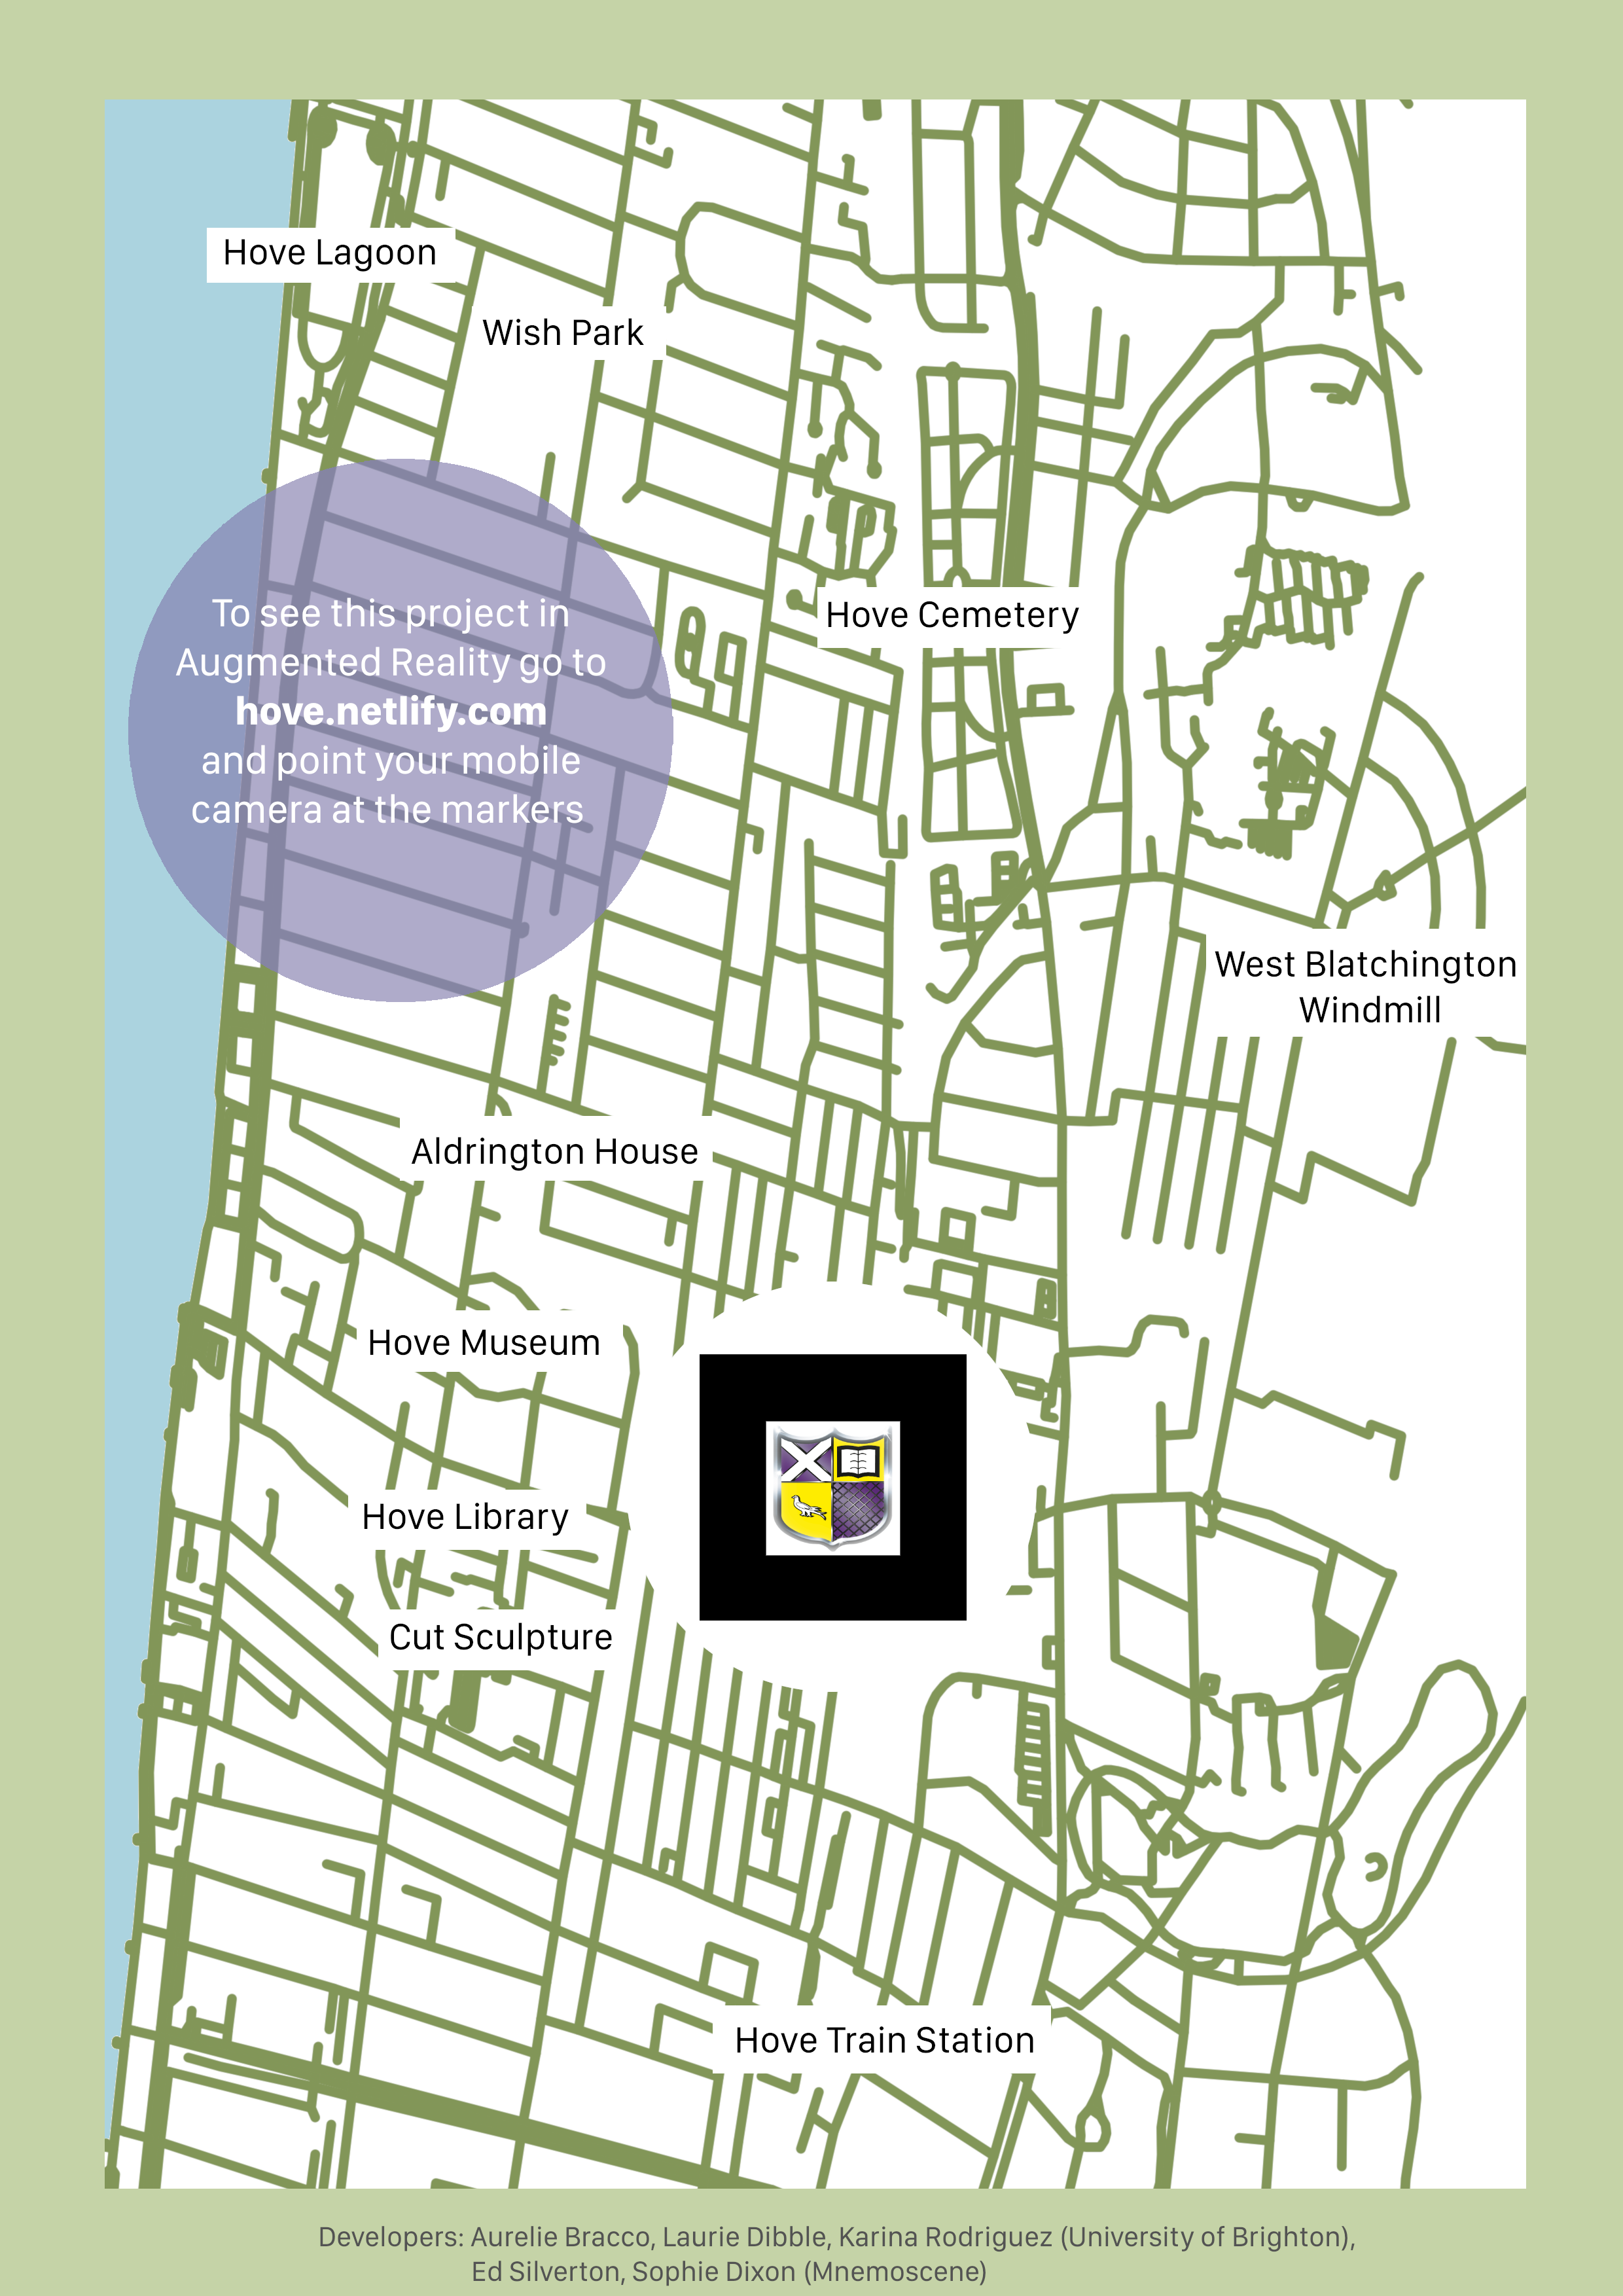
\includegraphics[width=0.49\linewidth]{images/side.png}
% \includegraphics[width=0.49\linewidth]{images/side1_cropped.png}
% \caption{Printed graphic for AR experience containing: left) rendered map by
% mapnik, AR pattern and instructions for access, and right) general information
% about the project} \label{fig:print} \end{figure*}



\end{document}
